%% LaTeX Template for ISIT 2025
%%
%% by Stefan M. Moser, October 2017
%% (with minor modifications by Tobias Koch, November 2023 and Michèle Wigger, November 2024)
%% 
%% derived from bare_conf.tex, V1.4a, 2014/09/17, by Michael Shell
%% for use with IEEEtran.cls version 1.8b or later
%%
%% Support sites for IEEEtran.cls:
%%
%% http://www.michaelshell.org/tex/ieeetran/
%% http://moser-isi.ethz.ch/manuals.html#eqlatex
%% http://www.ctan.org/tex-archive/macros/latex/contrib/IEEEtran/
%%

\documentclass[conference,letterpaper]{IEEEtran}
\usepackage{epsfig}
\usepackage{times}
\usepackage{float}
\usepackage{stfloats}
\usepackage{afterpage}

\usepackage{amstext,cite}
\usepackage{amssymb,bm}
\usepackage{latexsym}
\usepackage{color}
\usepackage{graphicx}


\usepackage{amsthm}
\usepackage{graphicx}
\usepackage[center]{caption}
\usepackage{pstricks}
%\usepackage{subfig}
\usepackage{caption}
\usepackage{subcaption}
\usepackage{booktabs}
\usepackage{multicol}
\usepackage{lipsum}% dummy text
\usepackage[T1]{fontenc}
%\UseRawInputEncoding
%\usepackage{mathabx}
\usepackage{hyperref}
 \usepackage{aecompl}
 \usepackage{mathrsfs}
\usepackage{arydshln}  % 导入用于虚线分隔的包




%
\setlength\unitlength{1mm}

\newcommand{\insertfig}[3]{
\begin{figure}[htbp]\begin{center}\begin{picture}(120,90)
\put(0,-5){\includegraphics[width=12cm,height=9cm,clip=]{#1.eps}}\end{picture}\end{center}
\caption{#2}\label{#3}\end{figure}}

\newcommand{\insertxfig}[4]{
\begin{figure}[htbp]
\begin{center}
\leavevmode \centerline{\resizebox{#4\textwidth}{!}{\input
#1.pstex_t}}
%\vspace*{-0.2in}
\caption{#2} \label{#3}
\end{center}
\end{figure}}

\long\def\comment#1{}

% bb font symbols

\newfont{\bbb}{msbm10 scaled 700}
\newcommand{\CCC}{\mbox{\bbb C}}

\newfont{\bb}{msbm10 scaled 1100}
\newcommand{\CC}{\mbox{\bb C}}
\newcommand{\PP}{\mbox{\bb P}}
\newcommand{\RR}{\mbox{\bb R}}
\newcommand{\QQ}{\mbox{\bb Q}}
\newcommand{\ZZ}{\mbox{\bb Z}}
\newcommand{\FF}{\mbox{\bb F}}
\newcommand{\GG}{\mbox{\bb G}}
\newcommand{\EE}{\mbox{\bb E}}
\newcommand{\NN}{\mbox{\bb N}}
\newcommand{\KK}{\mbox{\bb K}}

% Vectors

\newcommand{\av}{{\bf a}}
\newcommand{\bv}{{\bf b}}
\newcommand{\cv}{{\bf c}}
\newcommand{\dv}{{\bf d}}
\newcommand{\ev}{{\bf e}}
\newcommand{\fv}{{\bf f}}
\newcommand{\gv}{{\bf g}}
\newcommand{\hv}{{\bf h}}
\newcommand{\iv}{{\bf i}}
\newcommand{\jv}{{\bf j}}
\newcommand{\kv}{{\bf k}}
\newcommand{\lv}{{\bf l}}
\newcommand{\mv}{{\bf m}}
\newcommand{\nv}{{\bf n}}
\newcommand{\ov}{{\bf o}}
\newcommand{\pv}{{\bf p}}
\newcommand{\qv}{{\bf q}}
\newcommand{\rv}{{\bf r}}
\newcommand{\sv}{{\bf s}}
\newcommand{\tv}{{\bf t}}
\newcommand{\uv}{{\bf u}}
\newcommand{\wv}{{\bf w}}
\newcommand{\vv}{{\bf v}}
\newcommand{\xv}{{\bf x}}
\newcommand{\yv}{{\bf y}}
\newcommand{\zv}{{\bf z}}
\newcommand{\zerov}{{\bf 0}}
\newcommand{\onev}{{\bf 1}}

% Matrices

\newcommand{\Am}{{\bf A}}
\newcommand{\Bm}{{\bf B}}
\newcommand{\Cm}{{\bf C}}
\newcommand{\Dm}{{\bf D}}
\newcommand{\Em}{{\bf E}}
\newcommand{\Fm}{{\bf F}}
\newcommand{\Gm}{{\bf G}}
\newcommand{\Hm}{{\bf H}}
\newcommand{\Id}{{\bf I}}
\newcommand{\Jm}{{\bf J}}
\newcommand{\Km}{{\bf K}}
\newcommand{\Lm}{{\bf L}}
\newcommand{\Mm}{{\bf M}}
\newcommand{\Nm}{{\bf N}}
\newcommand{\Om}{{\bf O}}
\newcommand{\Pm}{{\bf P}}
\newcommand{\Qm}{{\bf Q}}
\newcommand{\Rm}{{\bf R}}
\newcommand{\Sm}{{\bf S}}
\newcommand{\Tm}{{\bf T}}
\newcommand{\Um}{{\bf U}}
\newcommand{\Wm}{{\bf W}}
\newcommand{\Vm}{{\bf V}}
\newcommand{\Xm}{{\bf X}}
\newcommand{\Ym}{{\bf Y}}
\newcommand{\Zm}{{\bf Z}}

% Calligraphic

\newcommand{\Ac}{{\cal A}}
\newcommand{\Bc}{{\cal B}}
\newcommand{\Cc}{{\cal C}}
\newcommand{\Dc}{{\cal D}}
\newcommand{\Ec}{{\cal E}}
\newcommand{\Fc}{{\cal F}}
\newcommand{\Gc}{{\cal G}}
\newcommand{\Hc}{{\cal H}}
\newcommand{\Ic}{{\cal I}}
\newcommand{\Jc}{{\cal J}}
\newcommand{\Kc}{{\cal K}}
\newcommand{\Lc}{{\cal L}}
\newcommand{\Mc}{{\cal M}}
\newcommand{\Nc}{{\cal N}}
\newcommand{\Oc}{{\cal O}}
\newcommand{\Pc}{{\cal P}}
\newcommand{\Qc}{{\cal Q}}
\newcommand{\Rc}{{\cal R}}
\newcommand{\Sc}{{\cal S}}
\newcommand{\Tc}{{\cal T}}
\newcommand{\Uc}{{\cal U}}
\newcommand{\Wc}{{\cal W}}
\newcommand{\Vc}{{\cal V}}
\newcommand{\Xc}{{\cal X}}
\newcommand{\Yc}{{\cal Y}}
\newcommand{\Zc}{{\cal Z}}

% Bold greek letters

\newcommand{\alphav}{\hbox{\boldmath$\alpha$}}
\newcommand{\betav}{\hbox{\boldmath$\beta$}}
\newcommand{\gammav}{\hbox{\boldmath$\gamma$}}
\newcommand{\deltav}{\hbox{\boldmath$\delta$}}
\newcommand{\etav}{\hbox{\boldmath$\eta$}}
\newcommand{\lambdav}{\hbox{\boldmath$\lambda$}}
\newcommand{\epsilonv}{\hbox{\boldmath$\epsilon$}}
\newcommand{\nuv}{\hbox{\boldmath$\nu$}}
\newcommand{\muv}{\hbox{\boldmath$\mu$}}
\newcommand{\zetav}{\hbox{\boldmath$\zeta$}}
\newcommand{\phiv}{\hbox{\boldmath$\phi$}}
\newcommand{\psiv}{\hbox{\boldmath$\psi$}}
\newcommand{\thetav}{\hbox{\boldmath$\theta$}}
\newcommand{\tauv}{\hbox{\boldmath$\tau$}}
\newcommand{\omegav}{\hbox{\boldmath$\omega$}}
\newcommand{\xiv}{\hbox{\boldmath$\xi$}}
\newcommand{\sigmav}{\hbox{\boldmath$\sigma$}}
\newcommand{\piv}{\hbox{\boldmath$\pi$}}
\newcommand{\rhov}{\hbox{\boldmath$\rho$}}

\newcommand{\Gammam}{\hbox{\boldmath$\Gamma$}}
\newcommand{\Lambdam}{\hbox{\boldmath$\Lambda$}}
\newcommand{\Deltam}{\hbox{\boldmath$\Delta$}}
\newcommand{\Sigmam}{\hbox{\boldmath$\Sigma$}}
\newcommand{\Phim}{\hbox{\boldmath$\Phi$}}
\newcommand{\Pim}{\hbox{\boldmath$\Pi$}}
\newcommand{\Psim}{\hbox{\boldmath$\Psi$}}
\newcommand{\Thetam}{\hbox{\boldmath$\Theta$}}
\newcommand{\Omegam}{\hbox{\boldmath$\Omega$}}
\newcommand{\Xim}{\hbox{\boldmath$\Xi$}}


% Sans Serif small case

\newcommand{\asf}{{\sf a}}
\newcommand{\bsf}{{\sf b}}
\newcommand{\csf}{{\sf c}}
\newcommand{\dsf}{{\sf d}}
\newcommand{\esf}{{\sf e}}
\newcommand{\fsf}{{\sf f}}
\newcommand{\gsf}{{\sf g}}
\newcommand{\hsf}{{\sf h}}
\newcommand{\isf}{{\sf i}}
\newcommand{\jsf}{{\sf j}}
\newcommand{\ksf}{{\sf k}}
\newcommand{\lsf}{{\sf l}}
\newcommand{\msf}{{\sf m}}
\newcommand{\nsf}{{\sf n}}
\newcommand{\osf}{{\sf o}}
\newcommand{\psf}{{\sf p}}
\newcommand{\qsf}{{\sf q}}
\newcommand{\rsf}{{\sf r}}
\newcommand{\ssf}{{\sf s}}
\newcommand{\tsf}{{\sf t}}
\newcommand{\usf}{{\sf u}}
\newcommand{\wsf}{{\sf w}}
\newcommand{\vsf}{{\sf v}}
\newcommand{\xsf}{{\sf x}}
\newcommand{\ysf}{{\sf y}}
\newcommand{\zsf}{{\sf z}}

% Sans Serif large case

\newcommand{\Asf}{{\sf A}}
\newcommand{\Bsf}{{\sf B}}
\newcommand{\Csf}{{\sf C}}
\newcommand{\Dsf}{{\sf D}}
\newcommand{\Esf}{{\sf E}}
\newcommand{\Fsf}{{\sf F}}
\newcommand{\Gsf}{{\sf G}}
\newcommand{\Hsf}{{\sf H}}
\newcommand{\Isf}{{\sf I}}
\newcommand{\Jsf}{{\sf J}}
\newcommand{\Ksf}{{\sf K}}
\newcommand{\Lsf}{{\sf L}}
\newcommand{\Msf}{{\sf M}}
\newcommand{\Nsf}{{\sf N}}
\newcommand{\Osf}{{\sf O}}
\newcommand{\Psf}{{\sf P}}
\newcommand{\Qsf}{{\sf Q}}
\newcommand{\Rsf}{{\sf R}}
\newcommand{\Ssf}{{\sf S}}
\newcommand{\Tsf}{{\sf T}}
\newcommand{\Usf}{{\sf U}}
\newcommand{\Wsf}{{\sf W}}
\newcommand{\Vsf}{{\sf V}}
\newcommand{\Xsf}{{\sf X}}
\newcommand{\Ysf}{{\sf Y}}
\newcommand{\Zsf}{{\sf Z}}


% mixed symbols

\newcommand{\sinc}{{\hbox{sinc}}}
\newcommand{\diag}{{\hbox{diag}}}
\renewcommand{\det}{{\hbox{det}}}
\newcommand{\trace}{{\hbox{tr}}}
\newcommand{\sign}{{\hbox{sign}}}
\renewcommand{\arg}{{\hbox{arg}}}
\newcommand{\var}{{\hbox{var}}}
\newcommand{\cov}{{\hbox{cov}}}
\newcommand{\SINR}{{\sf SINR}}
\newcommand{\SNR}{{\sf SNR}}
\newcommand{\Ei}{{\rm E}_{\rm i}}
\renewcommand{\Re}{{\rm Re}}
\renewcommand{\Im}{{\rm Im}}
\newcommand{\eqdef}{\stackrel{\Delta}{=}}
\newcommand{\defines}{{\,\,\stackrel{\scriptscriptstyle \bigtriangleup}{=}\,\,}}
\newcommand{\<}{\left\langle}
\renewcommand{\>}{\right\rangle}
\newcommand{\herm}{{\sf H}}
\newcommand{\trasp}{{\sf T}}
\newcommand{\transp}{{\sf T}}
\renewcommand{\vec}{{\rm vec}}
%\newcommand{\Psf}{{\sf P}}
%\newcommand{\mod}{{\rm mod}}

% equations
\newcommand{\be}{\begin{equation}}
\newcommand{\ee}{\end{equation}}
\newcommand{\bea}{\begin{eqnarray}}
\newcommand{\eea}{\end{eqnarray}}
\newtheorem{thm}{Theorem}%[section]
\newtheorem{cor}{Corollary}
\newtheorem{lem}{Lemma}
\newtheorem{prop}{Proposition}
\newtheorem{rem}{Remark}
\newtheorem{example}{Example}
\newtheorem{defn}{\protect\definitionname}

% Colors

\newcommand{\RED}{\color[rgb]{1.00,0.10,0.10}}
\newcommand{\BLUE}{\color[rgb]{0,0,0.90}}
\newcommand{\GREEN}{\color[rgb]{0,0.80,0.20}}

%%%%%%%%%%%%%%%%%%%%%%%%%%%%%%%%%%%%%%%%%%%%%%%%%
\def\MSE    {\mbox{\scriptsize\sf MSE}}
\def\Fsf{ {\sf F}}
\def\E{{\mathbb E}}
\def \Acomp {{A}}
\def\fsf{ {\sf f}}
\def\tr{{\rm tr}}
\def \Idm{{\bf I }}
\def\Var{{\rm Var}}
\def\pdf{{\rm p.d.f. }}

%% depending on your installation, you may wish to adjust the top margin:
\addtolength{\topmargin}{9mm}

%%%%%%
%% Packages:
%% Some useful packages (and compatibility issues with the IEEE format)
%% are pointed out at the very end of this template source file (they are 
%% taken verbatim out of bare_conf.tex by Michael Shell).
%
% *** Do not adjust lengths that control margins, column widths, etc. ***
% *** Do not use packages that alter fonts (such as pslatex).         ***
%
\usepackage[utf8]{inputenc} 
\usepackage[T1]{fontenc}
\usepackage{url}
\usepackage{ifthen}
\usepackage{cite}
\usepackage[cmex10]{amsmath} % Use the [cmex10] option to ensure complicance
                             % with IEEE Xplore (see bare_conf.tex)
\newcommand{\dt}[1]{{\blue #1}}
\newcommand{\NEW}[1]{{\red #1}}


\usepackage{amsmath}
\usepackage{tikz}
\usetikzlibrary{calc}

\usepackage[nodisplayskipstretch]{setspace} %\setstretch{1.5}
%% Please note that the amsthm package must not be loaded with
%% IEEEtran.cls because IEEEtran provides its own versions of
%% theorems. Also note that IEEEXplore does not accepts submissions
%% with hyperlinks, i.e., hyperref cannot be used.
% Define tikzmark and DrawboxF for multi-line box and labels
\newcommand{\tikzmark}[1]{\tikz[overlay,remember picture] \node (#1) {};}
% 定义第一个框命令 \DrawboxF
\newcommand{\DrawboxF}[4][]{%
    \tikz[overlay,remember picture]{%
        \coordinate (TopLeft)     at ($(#2)+(-0.2em,1.5em)$); % 调整顶部和底部坐标
        \coordinate (BottomRight) at ($(#3)+(0.2em,-2.5em)$); % 
        %
        \path (TopLeft); \pgfgetlastxy{\XCoord}{\IgnoreCoord};
        \path (BottomRight); \pgfgetlastxy{\IgnoreCoord}{\YCoord};
        \coordinate (LabelPoint) at ($(\XCoord,\YCoord)!0.5!(BottomRight)$);
        %
        \draw [#1, dashed] (TopLeft) rectangle (BottomRight); % 绘制虚线框
       \node [#1, fill=none, fill opacity=1] at ([xshift=-2em, yshift=-6pt]BottomRight.south) {#4};
    }
}

% 定义第二个框命令 \DrawboxV
\newcommand{\DrawboxV}[4][]{%
    \tikz[overlay,remember picture]{%
        \coordinate (TopLeft)     at ($(#2)+(-0.2em,1.5em)$);
        \coordinate (BottomRight) at ($(#3)+(0.2em,-3.5em)$); % 这里增加了下延伸距离
        %
        \path (TopLeft); \pgfgetlastxy{\XCoord}{\IgnoreCoord};
        \path (BottomRight); \pgfgetlastxy{\IgnoreCoord}{\YCoord};
        \coordinate (LabelPoint) at ($(\XCoord,\YCoord)!0.5!(BottomRight)$);
        %
        \draw [#1, dashed] (TopLeft) rectangle (BottomRight);
       \node [#1, fill=none, fill opacity=1] at ([xshift=-2em, yshift=-10pt]BottomRight.south) {#4};
    }
}

 \setlength {\marginparwidth }{2cm} 
 \newcommand{\DrawBox}[4][]{%
    \tikz[overlay,remember picture]{%
        \coordinate (TopLeft)     at ($(#2)+(-0.2em,0.9em)$);
        \coordinate (BottomRight) at ($(#3)+(0.2em,-0.3em)$);
        %
        \path (TopLeft); \pgfgetlastxy{\XCoord}{\IgnoreCoord};
        \path (BottomRight); \pgfgetlastxy{\IgnoreCoord}{\YCoord};
        \coordinate (LabelPoint) at ($(\XCoord,\YCoord)!0.5!(BottomRight)$);
        %
        \draw [red,#1] (TopLeft) rectangle (BottomRight);
        \node [below, #1, fill=none, fill opacity=1] at (LabelPoint) {#4};
    }
}

\interdisplaylinepenalty=2500 % As explained in bare_conf.tex


%%%%%%
% correct bad hyphenation here
\hyphenation{op-tical net-works semi-conduc-tor}

% ------------------------------------------------------------
\begin{document}
\title{On the Optimal Source Key Size of Secure Gradient Coding} 

% %%% Single author, or several authors with same affiliation:
% \author{%
%  \IEEEauthorblockN{Author 1 and Author 2}
% \IEEEauthorblockA{Department of Statistics and Data Science\\
%                    University 1\\
 %                   City 1\\
  %                  Email: author1@university1.edu}% }


%%% Several authors with up to three affiliations:
\author{%
  \IEEEauthorblockN{Yang Zhou, Wenbo Huang, Kai Wan, Robert Caiming Qiu}
  \IEEEauthorblockA{The School of Electronic Information and Communications,\\
                    Huangzhong University of Science and Technology,\\
                    430074 Wuhan, China\\
                    Email: \{hust\_zhou, eric\_huang, kai\_wan, caiming\}@hust.edu.cn}
  \and
  \IEEEauthorblockN{Claude E.~Shannon and David Slepian}
  \IEEEauthorblockA{Bell Telephone Laboratories, Inc.\\ 
                    Murray Hill, NJ, USA\\
                    Email: \{csh, dsl\}@bell-labs.com}
}

\author{
\IEEEauthorblockN{%
Yang Zhou\IEEEauthorrefmark{1},
Wenbo Huang\IEEEauthorrefmark{1},
Kai Wan\IEEEauthorrefmark{1},
Robert Caiming Qiu\IEEEauthorrefmark{1}
}
\IEEEauthorblockA{\IEEEauthorrefmark{1}Huazhong University of Science and Technology, 430074  Wuhan, China, \\ \{hust\_zhou, eric\_huang, kai\_wan, caiming\}@hust.edu.cn}%%
}


\maketitle

%%%%%%
%% Abstract: 
%% If your paper is eligible for the student paper award, please add
%% the comment "THIS PAPER IS ELIGIBLE FOR THE STUDENT PAPER
%% AWARD." as a first line in the abstract. 
%% For the final version of the accepted paper, please do not forget
%% to remove this comment!
%%

\begin{abstract}
With gradient coding, a user node can efficiently aggregate gradients from server nodes processing local datasets, achieving low communication costs and maintaining resilience against straggling servers.
This paper  considers secure gradient coding problem,
where a user aims to compute the sum of the gradients from ${\sf K}$ datasets with the assistance of ${\sf N}$ distributed servers. The user should recover the sum of gradients by the transmissions from any ${\sf N_r}$ servers, where each dataset is assigned to   $\Nsf-\Nsf_{\rm r}+\msf$ datasets. The security constraint guarantees that even if the user receives the transmission messages from all servers, it cannot obtain any other  information about the datasets  beyond the sum of gradients. 
It was shown in the literature that the security constraint will not increase the optimal communication cost of the gradient coding problem, if enough source keys are shared among the servers. 
However, the minimum  required  source key size to guarantee the security while achieving this optimal communication cost has only been studied for the case $\msf=1$. In this paper, we focus on the more general case $\msf\geq 1$, and aim to characterize the minimum  required  source key size for the above purpose.  
A new information-theoretic converse bound on the source key size 
and a new achievable scheme with smartly designed 
are proposed.  Our proposed scheme outperforms the optimal scheme with the widely-used cyclic data assignment  and coincides with the converse bound under some system parameters.
\end{abstract}

\section{Introduction}

Secure aggregation is a well-established topic in distributed computation, referring to the multiparty computation problem where the task is to compute a multiparty sum while no party reveals its update in the clear, not even to the aggregator~\cite{Bonawitz_Secure_Aggregation}. The concept of secret sharing was first introduced in \cite{shamir1979share}, where a secret is divided into multiple shares, and only participants meeting a threshold can reconstruct the secret. %Any group of participants below the threshold, even if they know the shares of multiple participants, cannot obtain any secret information, thereby ensuring information-theoretic security.
The complexity of verifiable secret sharing and its extension to multiparty computation were further studied in \cite{pedersen1991non, cramer2000complexity, ChaumMultiparty1988,yue2016healthcare}. 

In this paper, we consider the secure aggregation in gradient coding, called secure gradient coding. 
The gradient coding problem was first proposed in~\cite{pmlr-v70-tandon17a}. 
%which unified and extended the models of distributed gradient coding and distributed linear transformation~\cite{pmlr-v70-tandon17a,ye2018communication,Jahani2021OptimalCommunication-Computation,Short-dot}.
In a general gradient coding model, a user wants to compute a sum of gradients on   ${\sf K}$ datasets by ${\sf N}$ servers. During the data assignment phase, each dataset is assigned to $\Msf = \Nsf - \Nsf_{\rm r} + \msf$  servers.  During the computing phase, each server first computes gradients of the assgined datasets and then sends a coded message on these gradients to the user. During the decoding phase, the user should  recover the computation task result using the transmissions from any ${\sf N_r}$ servers. The objective is to minimize the number of transmissions (i.e., communication cost). 
In~\cite{ye2018communication}, the optimal communication cost under   linear encoding,  was characterized. 
%trade-off is explored between communication cost, computation load, and straggler tolerance in  distributed systems with homogeneous data assignment (i.e., each server is assigned by the same number of datasets). 
Furthermore, the authors in~\cite{Heterogeneous_Gradient_Coding} considers  heterogeneous (and arbitrarily fixed) data assignment, where each dataset may be assigned to different number of servers,  and 
characterizes the  optimal communication cost  under   linear encoding. 

The secure aggregation model for gradient coding was first proposed in~\cite{wan2022secure}.\footnote{\label{foot:linearly separable}The secure distributed linearly separable computation was formulated in~\cite{wan2022secure}. When the user only requests one linear combination of the gradients (or input vectors),  the problem reduces to secure gradient coding.} %and it closely resembles the model we consider in this work compared to other secure protocols. 
In this model, a key distribution server assigns a common shared key to all servers, in order to ensure  security.
It was proven in~\cite{wan2022secure} that the security constraint will not increase the optimal
communication cost of the gradient coding problem, if enough
source keys are shared among the servers. Then 
for the case  $\msf=1$ (i.e., when $\Msf$ is minimum to tolerate $\Nsf-\Nsf_{\rm r}$ stragglers), an information-theoretic lower bound on the source key size and  several secure distributed coded computation schemes for specific data distribution patterns (e.g., cyclic, repetitive, and mixed) were proposed in~\cite{wan2022secure},  while achieving the optimal communication cost with different requirement on the source key size. 


\iffalse
Secure gradient coding ensures that the user can only retrieve the sum of gradients without obtaining any additional information. Formally, it can be expressed as:
\begin{align}
I\left(g_{1}, \ldots, g_{\Ksf}; X_{[\Nsf]} \mid g_1 + \ldots + g_{\Ksf} \right) = 0, \label{eq:security}
\end{align}
where \( X_{[\Nsf]} \) denotes the encoded messages sent by all servers to the user. The secure gradient coding under minimum computation cost $ \msf = 1$ was first proposed in~\cite{wan2022secure}, and it discussed the minimum key size without increasing the communication cost.\footnote{The computation cost is defined as the number of datasets assigned to each server, while the communication cost is defined as the number of (coded) messages that the user should receive.}   
\fi 
 

Note that, recently,  secure aggregation for  federated learning has also gained significant attention \cite{fereidooni2021safe,choi2020communication, lightsecagg,jahani2022swiftagg,zhao2022information}. 
In secure aggregation for  federated learning, each distributed computing node holds its own local data to compute the gradient; thus secure aggregation against stragglers (or user dropouts) requires two-round transmissions. In contrast, in the gradient coding problem, an additional data assignment phase for servers exists, and because of the redundancy in data assignment, one-round transmission is enough for secure aggregation.

%achieves secure aggregation with only two rounds of communication, effectively reducing the communication cost. One of the bottlenecks of secure aggregation is key size. Based on the key size, the computation cost for key generation and the communication cost for key sharing will seriously influence the system computation capability. \cite{choi2020communication, jahani2022swiftagg} decrease the key size generated locally by each server, which in turn reduces both the computation cost and the communication cost between servers.

\iffalse
Key size is a crucial factor affecting both the computation cost and communication cost in secure aggregation, while individual key size influences the storage cost for each participant.
%{\red Why do we discuss the key size and individual key size? } 
In the secure distributed linearly separable computation problem, all keys are shared by a third trusted server to the servers~\cite{wan2022secure}. Since the demand matrix is constantly changing in real-time applications such as those in \cite{Yu_2021_ICCV} and convolution computations \cite{cong2014minimizing}, if we follow the key distribution method proposed in \cite{wan2022secure}, the third trusted server would need to broadcast all keys to the servers. In our proposed scheme, the third trusted server sends a unique key combination to each server at the beginning, independent of the demand matrix. It is clear that in our scheme, the third trusted server can perform key distribution without needing to know the demand.
This significantly reduces the communication cost for key sharing between the third trusted server and the servers and the storage cost for each server.
 Moreover, our scheme achieves the optimal individual key size with minimal communication cost. We also extend the scheme in \cite{wan2022secure} to make it work for general computation cost and provide the minimum key size.
 \fi
\paragraph*{Main Contributions} 
In this paper, we aim to characterize the minimum source key size for the case $\msf>1$, while achieving the optimal communication cost under   linear encoding.  Our main contributions are as follows.
\begin{itemize}
\item For a given data assignment, we provide an information-theoretic converse bound on the key size, while achieving the optimal communication cost under   linear encoding.
\item To reduce the key size, we introduce a  secure gradient coding  scheme with a new data assignment strategy. This scheme outperforms the widely used cyclic assignment scheme and can achieve the converse bound under some system parameters.
\iffalse
\item For any fixed data assignment, we propose an information-theoretic converse bound on the key size, while maintaining the optimal communication cost.   
\item To minimize the key size, we propose a new computing scheme with a novel assignment strategy. The computing scheme can cover the optimality results of the computational scheme with fractional repetition assignment; in general, it requires a smaller key size than the computing scheme with cyclic assignment while enabling optimal communication costs. 
\fi

%The new computing scheme is also applicable to the case of minimal computational cost in \cite{wan2022secure}.
\end{itemize}

\paragraph*{Notation Convention}
%We use the following notation convention.
Calligraphic symbols denote sets,  
bold lower-case letters denote vector, bold
upper-case letters denote matrices,
and sans-serif symbols denote system parameters.
We use $|\cdot|$ to represent the cardinality of a set or the length of a vector;
$[a:b]:=\left\{ a,a+1,\ldots,b\right\}$; %$(a:b]:=\{a+1,a+2,\ldots,b \} $, $[a:b):=\{a,a+1,\ldots,b-1 \} $, $(a,b)=\{a+1,a+2,\ldots,b-1\}$ and $[n] := [1:n]$; 
  $[n] := [1:n]$;
%$\oplus$ represents bit-wise XOR; $\mathbb{E}[\cdot]$ represents the expectation value of a random variable;  
%$a!=a\times (a-1) \times \ldots \times 1$ represents the factorial of $a$;
$\mathbb{F}_{\qsf}$ represents a  finite field with order $\qsf$;         
$\mathbf{M}^{\text{T}}$  and $\mathbf{M}^{-1}$ represent the transpose  and the inverse of matrix $\mathbf{M}$, respectively;
%$\text{rank}(\mathbf{M})$ represents the rank of matrix $\mathbf{M}$;
%$\mathbf{I}_n$ represents the identity matrix with dimension $n \times n$;
%${\bf 0}_{m \times n}$ represents the zero  matrix with dimension $m\times n$; 
 the matrix $[a;b]$ is written in a Matlab form, representing $[a,b]^{\text{T}}$;
$(\mathbf{M})_{m \times n}$ represents the dimension of matrix $\mathbf{M}$ is $m \times n$;
%$\mathbf{M}^{(\Sc)_{\rm r}}$ represents the sub-matrix of $\mathbf{M}$ which is composed of the rows  of $\mathbf{M}$ with indices in $\Sc$ (here $\rm r$ represents `rows'); 
%$\mathbf{M}^{(\Sc)_{\rm c}}$ represents the sub-matrix of $\mathbf{M}$ which is composed of the columns  of $\mathbf{M}$ with indices in $\Sc$ (here $\rm c$ represents `columns'); 
 %$\text{det}(\mathbf{M})$ represents the determinant matrix $\mathbf{M}$;
%$\mathbf{M}_{\Sc,\Vc}$ represents the sub-matrix of $\mathbf{M}$ by selecting from $\mathbf{M}$, the rows with indices in $\Sc$  and the columns with indices in $\Vc$.
 $\text{Mod} (b,a)$ represents the modulo operation on $b$ with  integer divisor $a$ and in this paper we let $\text{Mod}(b,a)\in \{1,\ldots,a \}$ (i.e., we let $ \text{Mod}(b,a)=a$ if $a$ divides $b$).
%$\text{GCD}(b,a)$ represents the Greatest Common Divisor of integers $b$ and $a$;   
%the number of $k$-permutations of $n, n\geq k,$ is indicated as $P(n,k):=n\cdot(n-1)\ldots(n-k+1)$.
%we let $\binom{x}{y}=0$ if $x<0$ or $y<0$ or $x<y$.
 %In this paper, for each set  of integers  $\Sc$, we sort the elements in $\Sc$ in an increasing order and denote the $i^{\text{th}}$ smallest element by $\Sc(i)$, i.e., $\Sc(1)<\ldots<\Sc(|\Sc|)$.

\section{System Model}
\label{sec:system}
This section describes   the $(\Ksf,\Nsf,\Nsf_{\rm r}, \msf)$ secure gradient coding problem. 
We consider the framework that a user computes the sum of gradients on $\Ksf$ independent datasets $D_1,\ldots, D_{\Ksf}$ with the help of ${\sf N}$ servers. %$D_i\in \mathbb{R}^\Lsf$. 
\iffalse
Due to the large volume of data, the computational tasks are distributed across $\Nsf$ servers. Each dataset is stored in ${\sf M}$ different servers. The collection of datasets assigned to server $n \in [{\sf N}]$ is denoted as $\Zc_n$. Server $n$ computes the gradient $g_{i} \in \mathbb{F}^{\Lsf}_{\qsf}$ of the assigned dataset  $D_{i}$,  where $i \in \Zc_{n}$, and sends coded message $X_{n}$ in terms of its computed  gradients and stored keys. 

%the linear combinations of the gradients and keys to the user which denotes as coded message $X_{n}.$ 
 %On the straggler effect, 
 We define ${\sf N_r}$ as  the number of minimum available servers. The user should recover the aggregated gradient $g_{1} + \cdots + g_{\sf N}$, by receiving  the coded messages from any ${\sf N_r}$  servers.
 \fi 
\iffalse
We consider the security aggregation of distributed linearly separable computation over the canonical user-server distributed system, originally proposed in~\cite{wan2022secure}. 

The user computes a linearly separable function of $\Ksf$  datasets $D_1, \ldots, D_{\Ksf}$, with the help of $\Nsf$ servers without obtaining any other information about datasets. The computation task can be written as $\Ksf_{\rm c}$ linear combinations of $\Ksf$ messages
\begin{align}
    &f({D_1},{D_2}, \ldots ,{D_{\Ksf}}) = g({f_1}({D_1}), \ldots ,{f_{\Ksf}}({D_{\Ksf}}))  \nonumber\\
    &= g({W_1}, \ldots ,{W_{\Ksf}}) = {\bf F}[{W_1}; \ldots ;{W_\Ksf}] = [{F_1};\ldots;{F_{\Ksf_{\rm c}}}], \label{eq:computation task}
\end{align}
where the $i^{\text{th}}$ message is  ${W_i} = {f_i}({D_i}) $, representing  the outcome of the  component function $f_i(\cdot)$ applied to dataset $D_i$. Each message $W_i$ contains $\Lsf$ uniformly i.i.d. symbols in $\mathbb{F}_{\qsf}$ for some large enough prime-power $\qsf$. ${\bf F}$ represents the demand matrix with dimension $\Ksf_{\rm c} \times \Ksf$, where each element is uniformly i.i.d. over $\mathbb{F}_{\qsf}$\footnote{\label{foot:L large}In this paper, we assume that  $\Ksf/\Nsf$ is an integer and  $\Lsf$ is large enough such
that any sub-message division is possible. We only consider $\Ksf_{\rm c} \leq \Ksf$ because when $\Ksf_{\rm c} \le \Ksf,$  $\text{Rank}({\bf F}) = \Ksf_{\rm c}$ with high probability and when $\Ksf_{\rm c} > \Ksf,$ $\text{Rank}({\bf F}) = \Ksf$ with high probability, we only consider the non-trivial setting $\Ksf_{\rm c} \le \Ksf$}. 

To tolerate $\Nsf - \Nsf_{\rm r}$ stragglers, the user can complete the computation task from any $\Nsf_{\rm r}$ servers' messages. Each server is assigned $\Msf = \frac{\Ksf}{\Nsf} (\Nsf - \Nsf_{\rm r} + \msf ) $ datasets, where $\Msf$ is defined as the computation cost and $\msf$ is a communication reduction factor.

\fi
 Compared to distributed computing without considering secure aggregation, there is another trusted  server to distribute keys to the computing servers. It generates a set of  random variables $\Qc = \{Q_{1}, \ldots, Q_{\Nsf}\}$ on $\mathbb{F}_{\qsf}$ indepndent of the datasets, %and then assigns them to servers based on indices. Thus    
\begin{align}
I(Q_1, \ldots, Q_{\Nsf} ; D_1, \ldots, D_{\Ksf} ) = 0. \label{eq:independent key}
\end{align}
The source key size \( \eta \) measures the total amount of randomness among all keys, i.e.,
\begin{align}
\eta = H( Q_1, \ldots, Q_{\Nsf} )/\Lsf. \label{eq:def of eta}
\end{align}


The secure gradient coding framework comprises three phases, {\it data assignment, computing, and decoding}. 

{\it Data assignment phase.}
The data center assigns each dataset to $\Msf =\Nsf-\Nsf_{\rm r}+\msf$ servers, where $\msf$ is  computation cost factor (which is also called communication reduction factor in~\cite{ye2018communication}). The index set of datasets assigned to server $n \in [{\sf N}]$ is denoted as $\Zc_n \in [\Ksf]$.  In addition, the trusted key server allocates the key   $\Qc_i$ to each server $i\in [\Nsf]$.


%Server $n$ computes the gradient $g_{i} \in \mathbb{F}^{\Lsf}_{\qsf}$ of the assigned dataset  $D_{i}$,  where $i \in \Zc_{n}$, and sends coded message $X_{n}$ in terms of its computed  gradients and stored keys. 

{\it Computing phase.}
Each server $n \in[\Nsf]$ first computes the message $g_k = \nabla (D_k)$ for each $k \in \Zc_n$. Then it sends the coded message to the user, 
\begin{align}
 X_n = \psi_n \left( \{g_k:  k \in \Zc_n\},  Q_n \right),
 \end{align}
  where  $\psi_n$  is a  function of messages $\{g_k: k\in \Zc_n\}$, 
\begin{align} 
\psi_n &:  \mathbb{F}_{\qsf}^{ |\Zc_n| \Lsf} \times   | \Qc |  \to \mathbb{F}_{\qsf}^{ \Tsf_n },  
\label{eq: encoding function def}
\end{align}
and $\Tsf_n$ represents the length of $ X_n $. %Finally, server $n$ transmits $X_n$ to the user. 
%$|\Zc_n|$ is denoted as the computation cost 
$\msf$ is the computation cost factor because  in a distributed system, the complexity of computing the linear combinations of the gradients is much lower than computing the gradients. %So, the computation cost can be represented by the number of messages each server computes.

{\it Decoding phase.}
 We define ${\sf N_r}$ as  the number of minimum available servers, and the identity of the surviving servers is not known until the decoding phase. 
Thus the user should be able to use coded messages from any $\Nsf_{\rm r}$  servers to decode the computation tasks. 
Thus, for each subset of servers $\Ac \subseteq [\Nsf]$ where $|\Ac| = \Nsf_{\rm r}$, by defining
$
    {X_{\Ac}}: = ( {X_n}:n \in \Ac), 
$
it should satisfy that
\begin{align}
    H(g_1+\ldots+g_K | X_{\Ac}) = 0.
\end{align}
\iffalse
there should be a decoding function such that 
$
\hat{g}_{\Ac}= \phi_{\Ac}\big( X_{\Ac}, {\bf F} \big),
$
where 
\begin{align}
    {\phi _\Ac}: \mathbb{F}_{\qsf}^{\sum_{n \in \Ac}{\Tsf_{\rm n}}} \times {\mathbb{F}_{\qsf}}^{{\Ksf_{\rm c}}\times \Ksf} \to {\mathbb{F}_{\qsf}}^{{\Ksf_{\rm c}}\times \Lsf}.
\end{align}


The  worst-case error probability is defined as
\begin{align}
 \varepsilon:= \max_{\Ac  \subseteq [\Nsf]: |\Ac|= \Nsf_{\rm r}} \Pr\{ \hat{g}_{\Ac} \neq g(W_1,   \ldots, W_{\Ksf}) \}. 
\end{align}
A computing scheme is called achievable if   the  worst-case     
error probability vanishes when $\qsf \to \infty$. 
\fi

We define 
\begin{equation}
    \Rsf: = \mathop {\max }\limits_{\Ac \subseteq [\Nsf]:|\Ac| = {\Nsf_{\rm r}}} \frac{{\sum\nolimits_{n \in \Ac} {{\Tsf_n}} }}{\Lsf}
\end{equation} 
as the communication cost, which represents the maximum normalized number of symbols received from any $\Nsf_{\rm r}$ servers to recover the computational task.

The secure aggregation protocol imposes that  
\begin{align}
    I\left(g_{1},\ldots, g_{\Ksf};   X_{[\Nsf]} | g_1+\ldots+g_{\Ksf}  \right) = 0,
\end{align}
where $X_{[\Nsf]}$ presents the whole messages from $\Nsf$ servers which may be received by the user. This equation ensures that, except for the computation task, the user cannot obtain any information about the datasets.

If the source key size is large enough, the optimal communication cost under linear encoding (i.e., $ \psi_n$ is a  linear function), can be  characterized by  directly combining~\cite{wan2022secure,ye2018communication}.\footnote{\label{foot:direct optimal}Without  security, the authors in \cite{ye2018communication} characterized  the optimal communication cost  under linear encoding  is $\Nsf_{\rm r}/\msf$. In addition,~\cite[Theorem 1]{wan2022secure} showed that for any $(\Ksf, \Nsf, \Nsf_{\rm r}, \msf)$ non-secure gradient coding problem, the coding scheme can be made secure without increasing the communication cost.} 
\begin{thm}[\cite{wan2022secure,ye2018communication}]
\label{thm:communication cost}
For the  $(\Ksf,\Nsf,\Nsf_{\rm r}, \msf)$ secure gradient coding problem, the optimal communication cost under linear encoding is 
$ \frac{\Nsf_{\rm r}}{\msf}$
\end{thm}



Our main objective in this paper is to minimize the source key size $\eta$ while maintaining the optimal communication cost under linear encoding  for the case $ \msf \geq 1$.

%the optimal communication cost, and minimize the key size $\eta$ while maintaining the optimal communication cost in the case where $ \msf \geq 1$.






\section{Main Results}
\label{sec:main}
%In the following, we present our main results.
We first introduce a novel converse bound on $ \eta $ for a fixed assignment, {\red whose proof can be found in the extended version of this paper~\cite[Appendix ????]{GITHUB}.}
\begin{thm}
\label{thm:bound of η}
For the $(\Ksf,\Nsf,\Nsf_{\rm r}, \msf)$ secure gradient coding problem, for a fixed assignment \(\mathbf{Z} = (\Zc_1, \ldots, \Zc_{\Nsf})\), if there exists an ordered set of servers in \([\Nsf]\), denoted by \(\sv = (s_1, \ldots, s_{|\sv|})\), where each server contains at least one dataset that appears in the datasets of its preceding servers at most \(\msf - 1\) times, this can be expressed as:
\begin{align}
\forall i \in [|\sv|], \exists x \in \Zc_{s_i} \text{ such that } \sum_{j=1}^{i-1} \delta(x \in \Zc_{s_j}) \leq \msf - 1, \label{eq:vector constraint}
\end{align}
where \(\delta(x \in \Zc_{s_j})\) equals \(1\) if \(x \in \Zc_{s_j}\), and \(0\) otherwise.

It must hold that
\begin{align}
\eta \geq \frac{|\sv|}{\msf}-1. \label{eq:converse lemma}
\end{align}
\end{thm}
Theorem~\ref{thm:bound of η} indicates that minimizing key size $\eta$ is a combinatorial problem that depends on the data assignment. 
Further, we can establish a min-max problem to characterize the minimum $\eta^{\star}$ as follows.
\begin{cor}
    For the $(\Ksf,\Nsf,\Nsf_{\rm r}, \msf)$ secure gradient coding problem, we have
    \begin{align}
\eta^{\star} \geq \min_{\mathbf{Z}}
\max_{\sv \subseteq [\Nsf], ~\text{subject to}~ \eqref{eq:vector constraint} } \frac{|\sv|}{\msf}-1. \label{eq:converse lemma}
\end{align}
\end{cor}

The essence of min-max problems lies in balancing extreme values across all chosen $\sv$.\footnote{According to the extremal principle, if there exists a data assignment method that equalizes or minimizes the differences in the objective function values, such an assignment is typically globally optimal. Thus, we would like to divide the servers into different groups and make servers in the same group assigned datasets as similar as possible.} In order to simplify the computation, we provide a loosen converse bound on $\eta^{\star}$, {\red whose proof could be found in~\cite[Appendix ???]{GITHUB}.}
%whose $|\sv|$ are equal in Corollary~\ref{cor:converse cor}, and propose an achievable scheme in Theorem~\ref{thm:main achievable scheme}. 

\begin{cor}
\label{cor:converse cor}
For the $(\Ksf,\Nsf,\Nsf_{\rm r}, \msf)$ secure gradient coding problem,
% to achieve the optimal communication cost, 
 it must hold that
\begin{align}
\eta^{\star} \geq \frac{\left\lceil  \frac{\msf\Nsf}{\Nsf-\Nsf_{\rm r}+\msf} \right\rceil}{\msf} -1. \label{eq:converse cor}
\end{align}
\end{cor} 
      


Next, we propose a novel secure gradient coding scheme that employs a new data assignment strategy, improving the commonly used cyclic  assignment.

\begin{thm}
\label{thm:main achievable scheme}
For the $(\Ksf,\Nsf,\Nsf_{\rm r}, \msf)$ secure gradient coding problem, the source key size  $\eta=  \frac{ h(\Nsf,\Msf)}{\msf}-1$ is achievable, where the output of the function \( h(\cdot, \cdot) \) is given by the recursive algorithm shown in Fig.~\ref{fig:scheme} with the following properties:
 \begin{itemize}

 \item When  $\Nsf > 2\Msf$,  by {\it Scheme~1} described in Section~\ref{sub:partial rep} we have  
\begin{align}
h(\Nsf,\Msf)=h\big(\Nsf-\left\lfloor \Nsf/\Msf-1\right\rfloor \Msf,\Msf\big)+ \msf\left\lfloor \Nsf/\Msf -1\right\rfloor  . \label{eq:from partial rep}
\end{align} 
\item When $1.5 \Msf \leq \Nsf < 2 \Msf$ and $\Msf$ is even, with $\Msf \geq 2\msf$,
by {\it Scheme~2} described in Section~\ref{sub:M is even}, we have  
\begin{align}
 h(\Nsf, \Msf) = h\left(\Nsf - \Msf, \frac{\Msf}{2}\right) + \msf. \label{eq:M is even}
\end{align}

 \item When $1.5 \Msf \leq  \Nsf < 2 \Msf$ and $\Msf$ is odd, with $\Msf \geq 2\msf+1$, by  {\it Scheme~3} described in Section~\ref{sub:M is odd} we have  
 \begin{align}
 h(\Nsf,\Msf)=   \Nsf-\frac{3\Msf-1}{2}+2 \msf; \label{eq:M is odd}
 \end{align}
 \item When $\Msf< \Nsf <  1.5 \Msf$, with $\Msf \geq 2\msf$, by  {\it Scheme~4} described in Section~\ref{sub:less than 1.5M}  we have  
\begin{align}
h(\Nsf,\Msf)=h(\Msf,2\Msf-\Nsf). \label{eq:less than 1.5M}
\end{align} 
  \end{itemize}
    \hfill $\square$ 
 \end{thm} 
Notice that $\lambda$ in Fig.~\ref{fig:scheme} represents the number of totally transmitted linearly independent combinations of merged messages, and we aim to minimize it.
 
\begin{rem}[The key size in extreme cases]
\label{rem:extreme cases}
\em

For the $(\Ksf,\Nsf,\Nsf_{\rm r}, \msf)$ secure gradient coding problem with  $\Msf= \Nsf - \Nsf_{\rm r} + \msf$, and $\Msf$ divides $\Nsf$, the minimum key size is
\begin{align}
    \eta^{\star} = \frac{\Nsf}{\Msf} - 1, \label{eq:gradient eta rho rep}
\end{align}
which matches the converse~\eqref{cor:converse cor} and is achievable using fractional repetition assignment.

Under the cyclic assignment constraint, the minimum key size required for optimal communication cost is
\begin{align}
    \eta^{\star}_{\text{cyc}} = \frac{\Nsf_{\rm r}}{\msf} - 1. \label{eq:gradient eta cyc}
\end{align}


\end{rem}

\iffalse
\begin{rem}[Simplification idea of Theorem~\ref{thm:main achievable scheme}]
\label{M'=M}
We divide the $\Ksf$ datasets into $\Nsf$ non-overlapping, equal-length groups, where the $i^{\text{th}}$ group, $\Gc_i = \{k \in [\Ksf] : \text{Mod}(k, \Nsf) = i\}$, contains $\frac{\Ksf}{\Nsf}$ datasets for each $i \in [\Nsf]$. Each group $\Gc_i$ is assigned to $\Msf = \Nsf - \Nsf_{\rm r} + \msf$ servers, which compute the merged message $W^{\prime}_i$. Thus, we reduce the $(\Ksf, \Nsf, \Nsf_{\rm r}, 1, \Msf)$ secure distributed linearly separable computation problem to the $(\Nsf, \Nsf, \Nsf_{\rm r}, 1, \Msf)$ problem.
\end{rem}
\fi


At the end of this section, we present numerical evaluations comparing the key size in converse in~\eqref{eq:converse cor}, in the cyclic assignment scheme, and in the scheme from Theorem~\ref{thm:main achievable scheme}. %In Fig.~\ref{fig:numerical 1b}, we fix $\Msf = 6, \msf = 2$ and show the tradeoff between $\Nsf$ and $\eta$. In Fig.~\ref{fig:numerical 1c}, we fix $\Nsf = 24, \Msf = 10$ and show the tradeoff between $\msf$ and $\eta$. 
The results demonstrate that the combined scheme requires a significantly smaller key size than the cyclic assignment scheme and coincides with the relaxed converse at some points.


\begin{figure*}%[ht]
%\vspace{-2mm}
\centerline{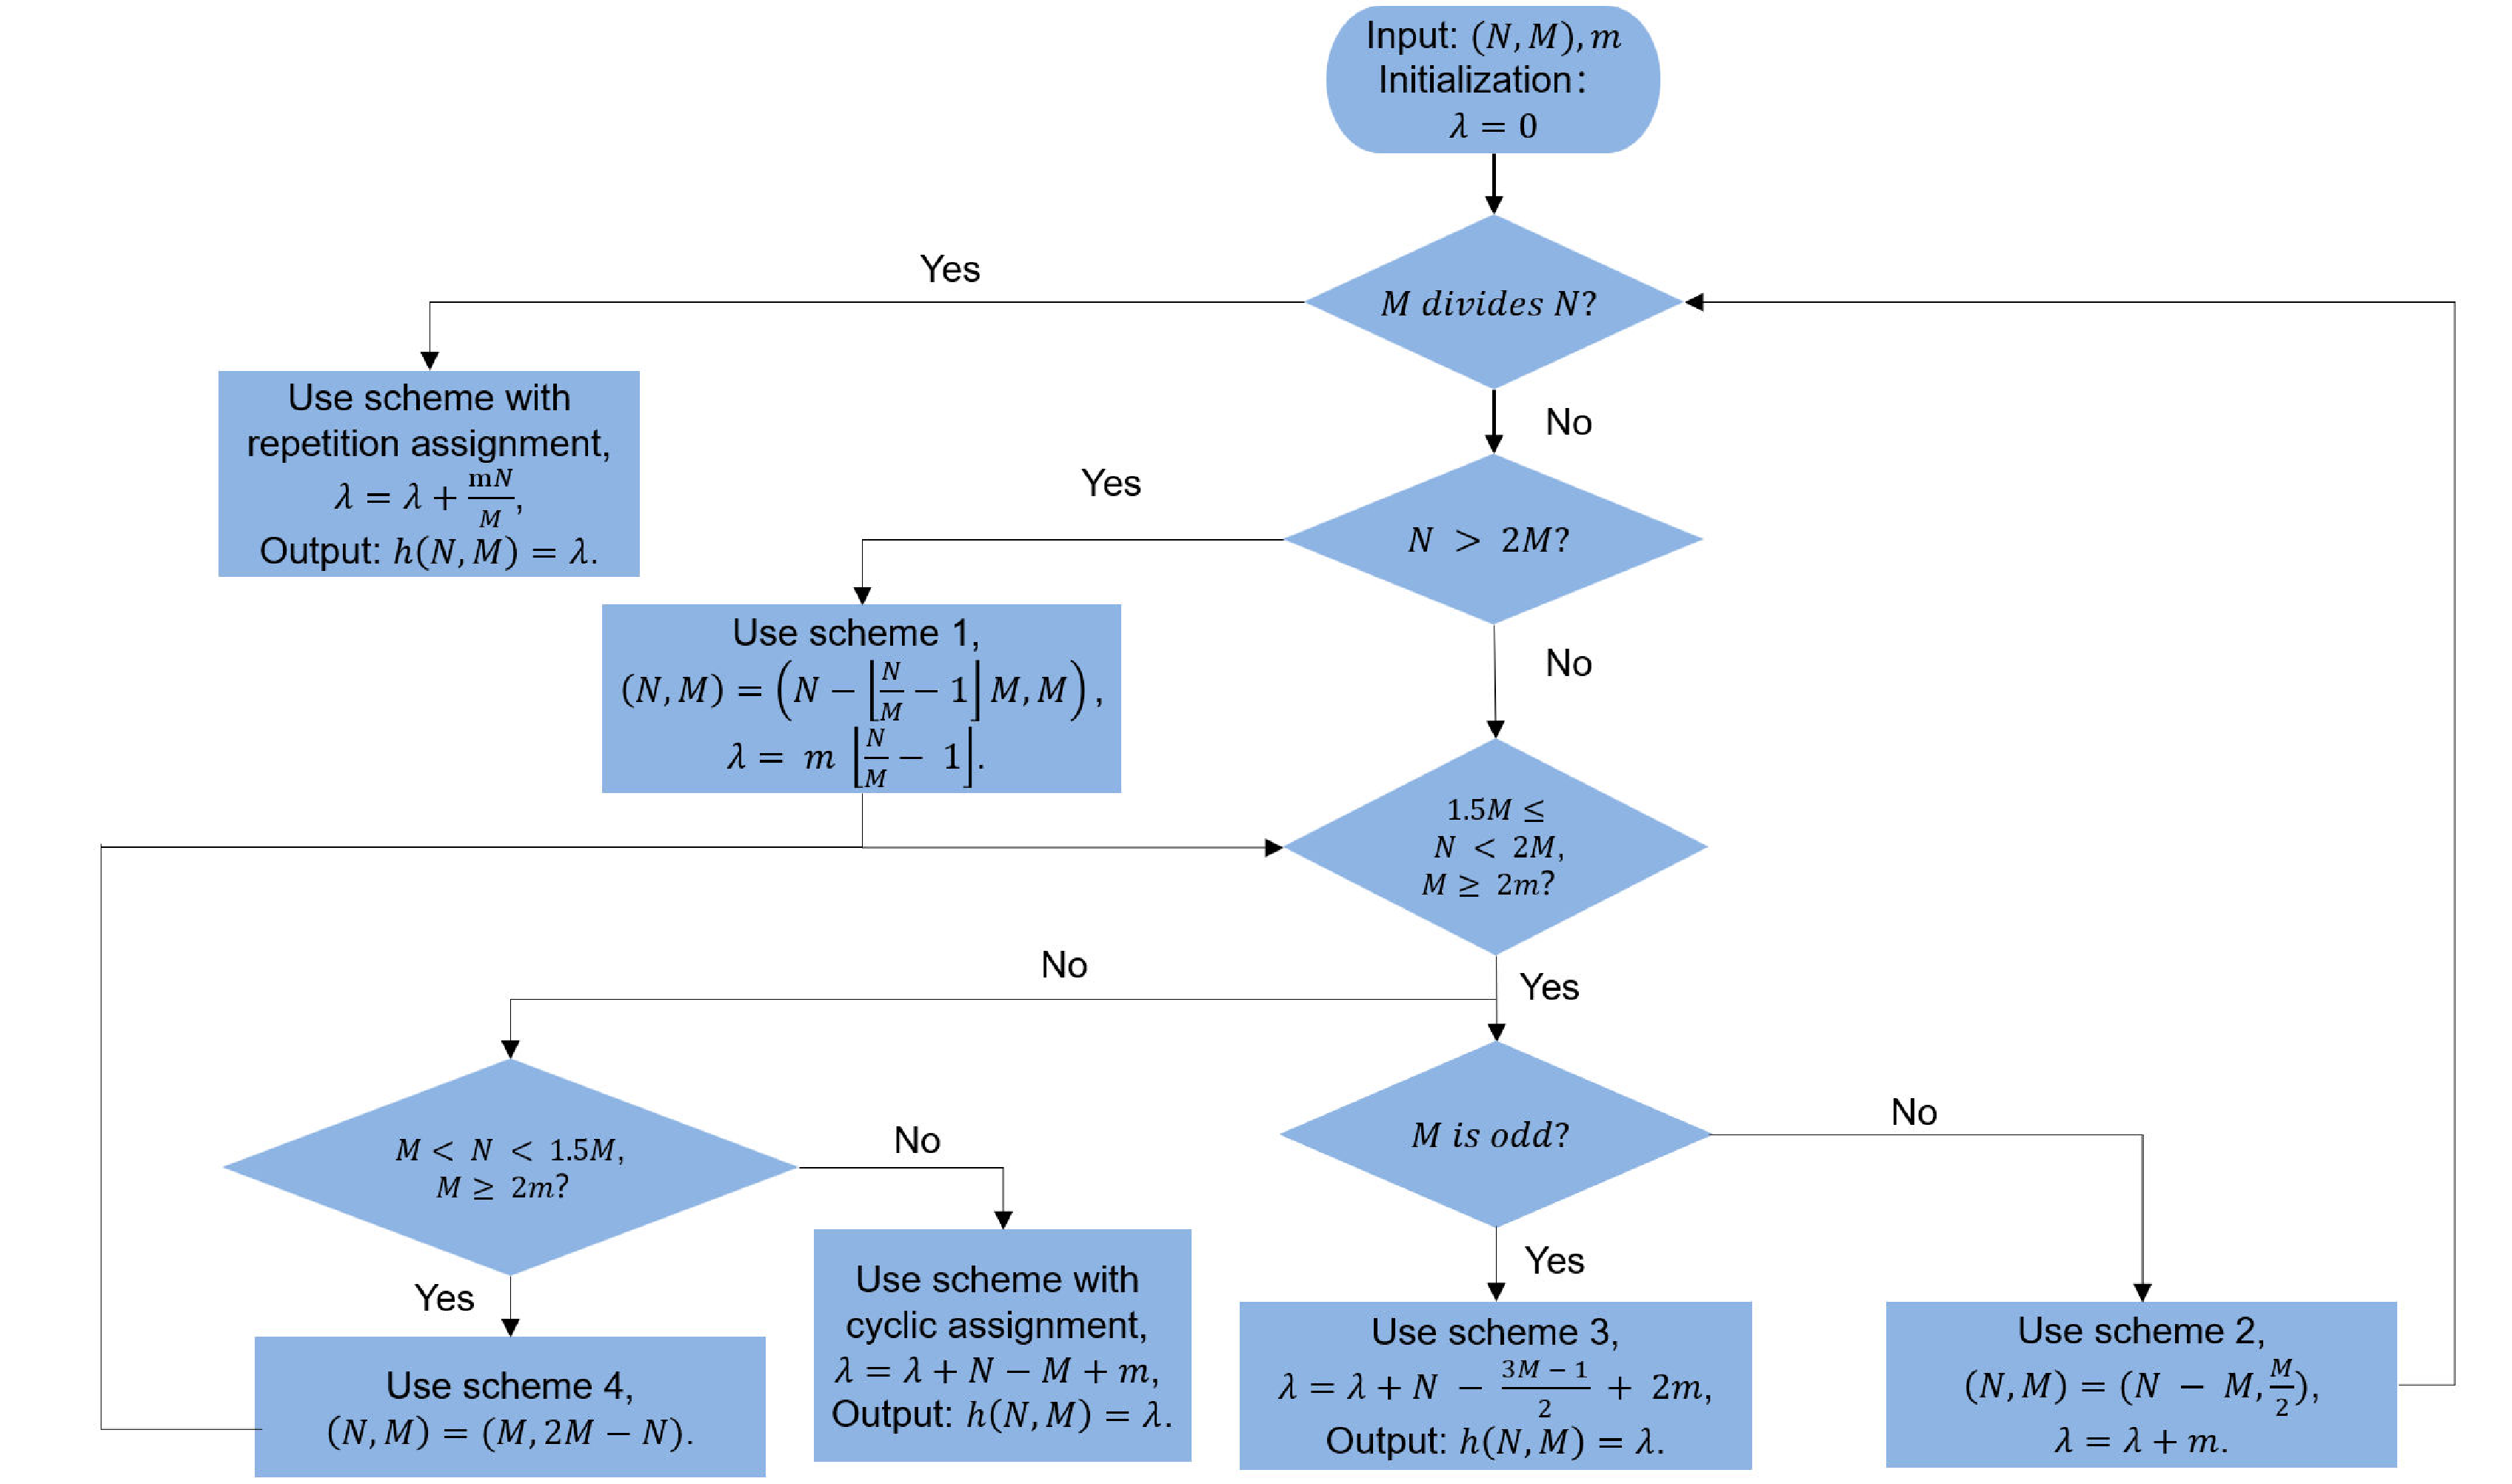
\includegraphics[scale=0.25]{scheme}}
\caption{\small Flow diagram of the combined scheme in Theorem~\ref{thm:main achievable scheme}.}
\label{fig:scheme} % 创建分割线
%\vspace{-5mm}
\end{figure*}


\begin{figure}[ht] 
    \centering
    \iffalse
    \begin{subfigure}[t]{0.5\textwidth}
        \centering
        \includegraphics[scale=0.45]{M varies.pdf}
        \caption{\small $(\Msf,\eta)$ tradeoff with $\Nsf=24$ and $\msf=2$.}
        \label{fig:numerical 1a}
    \end{subfigure}\\
    \fi
    \begin{subfigure}[t]{0.5\textwidth}
        \centering
        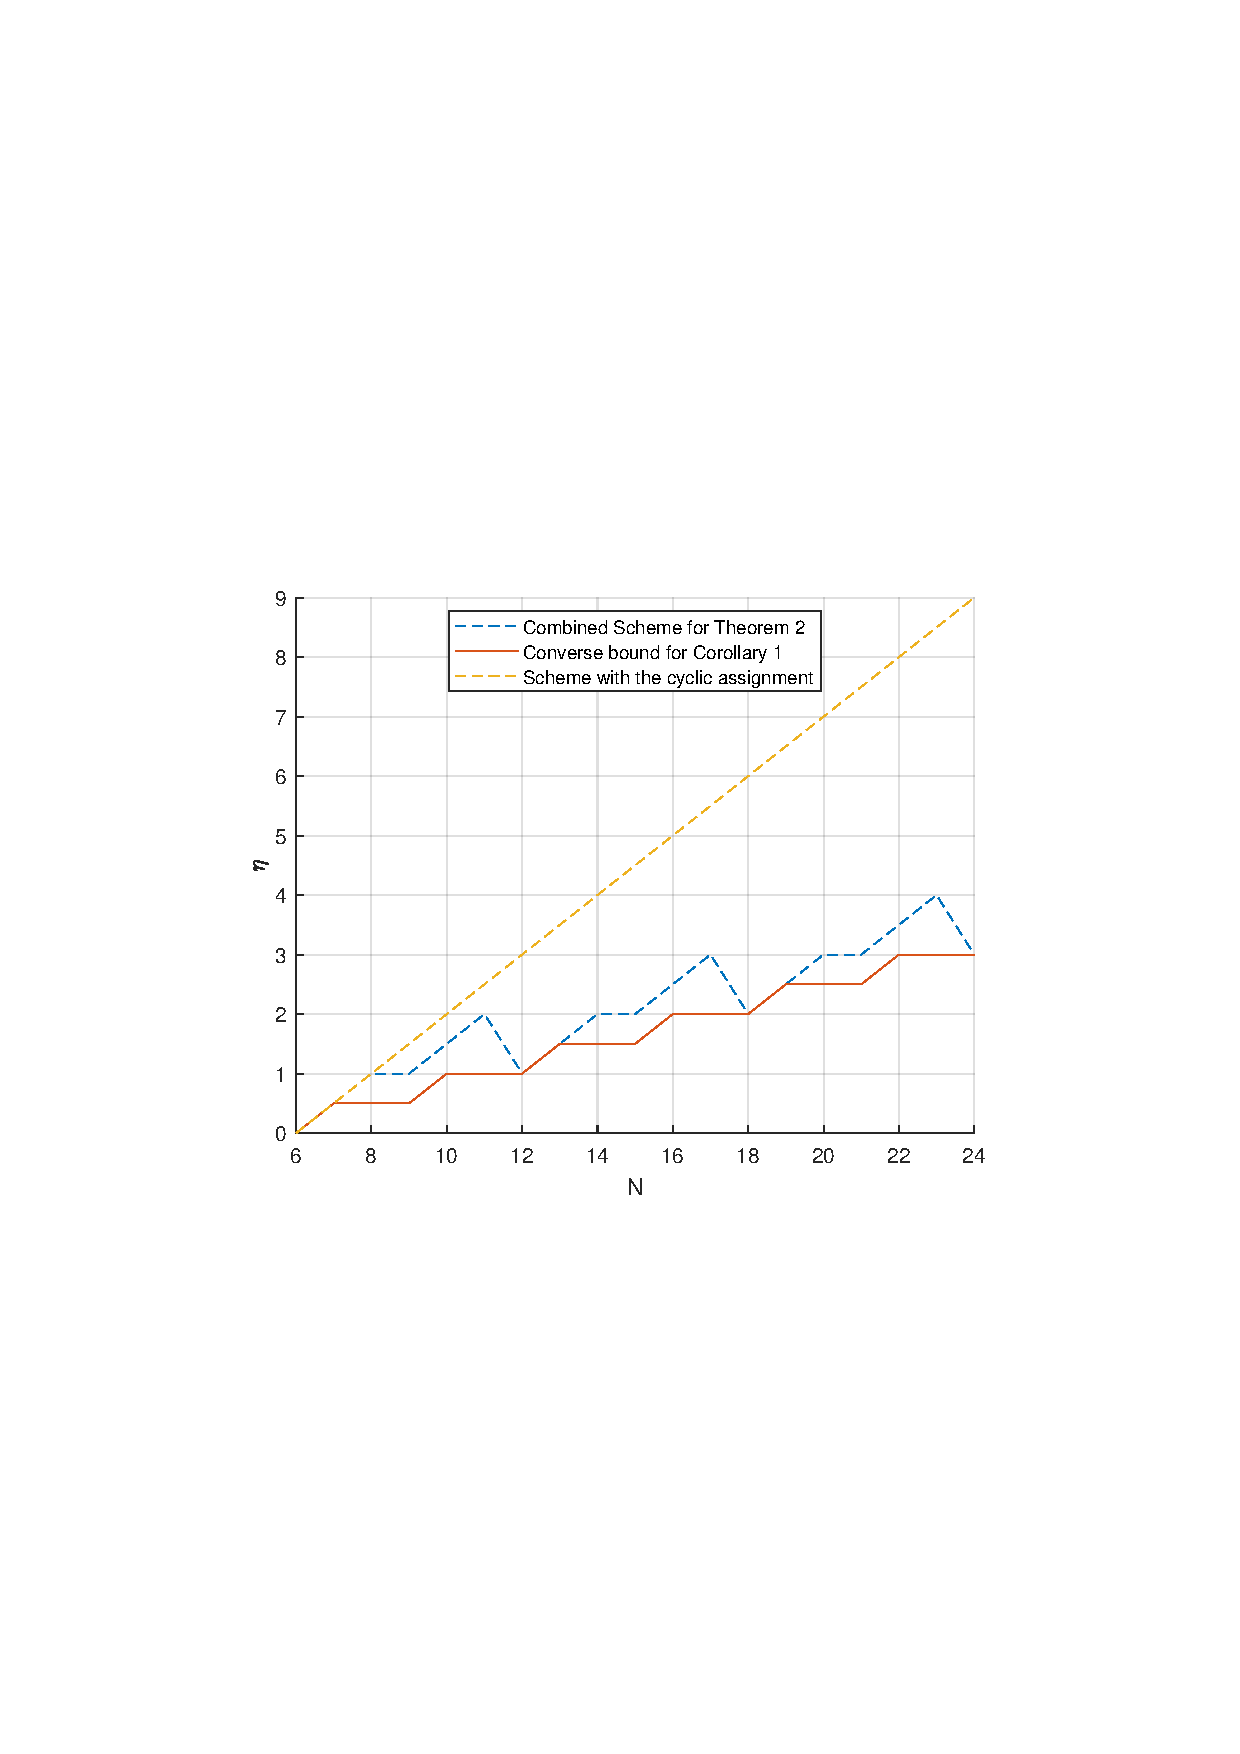
\includegraphics[scale=0.45]{N varies.pdf}
        \caption{\small $(\Nsf,\eta)$ tradeoff with $\Ksf = \Nsf, \Msf=6, \msf=2$.}
        \label{fig:numerical 1b}
    \end{subfigure}\\
    \begin{subfigure}[t]{0.5\textwidth}
        \centering
        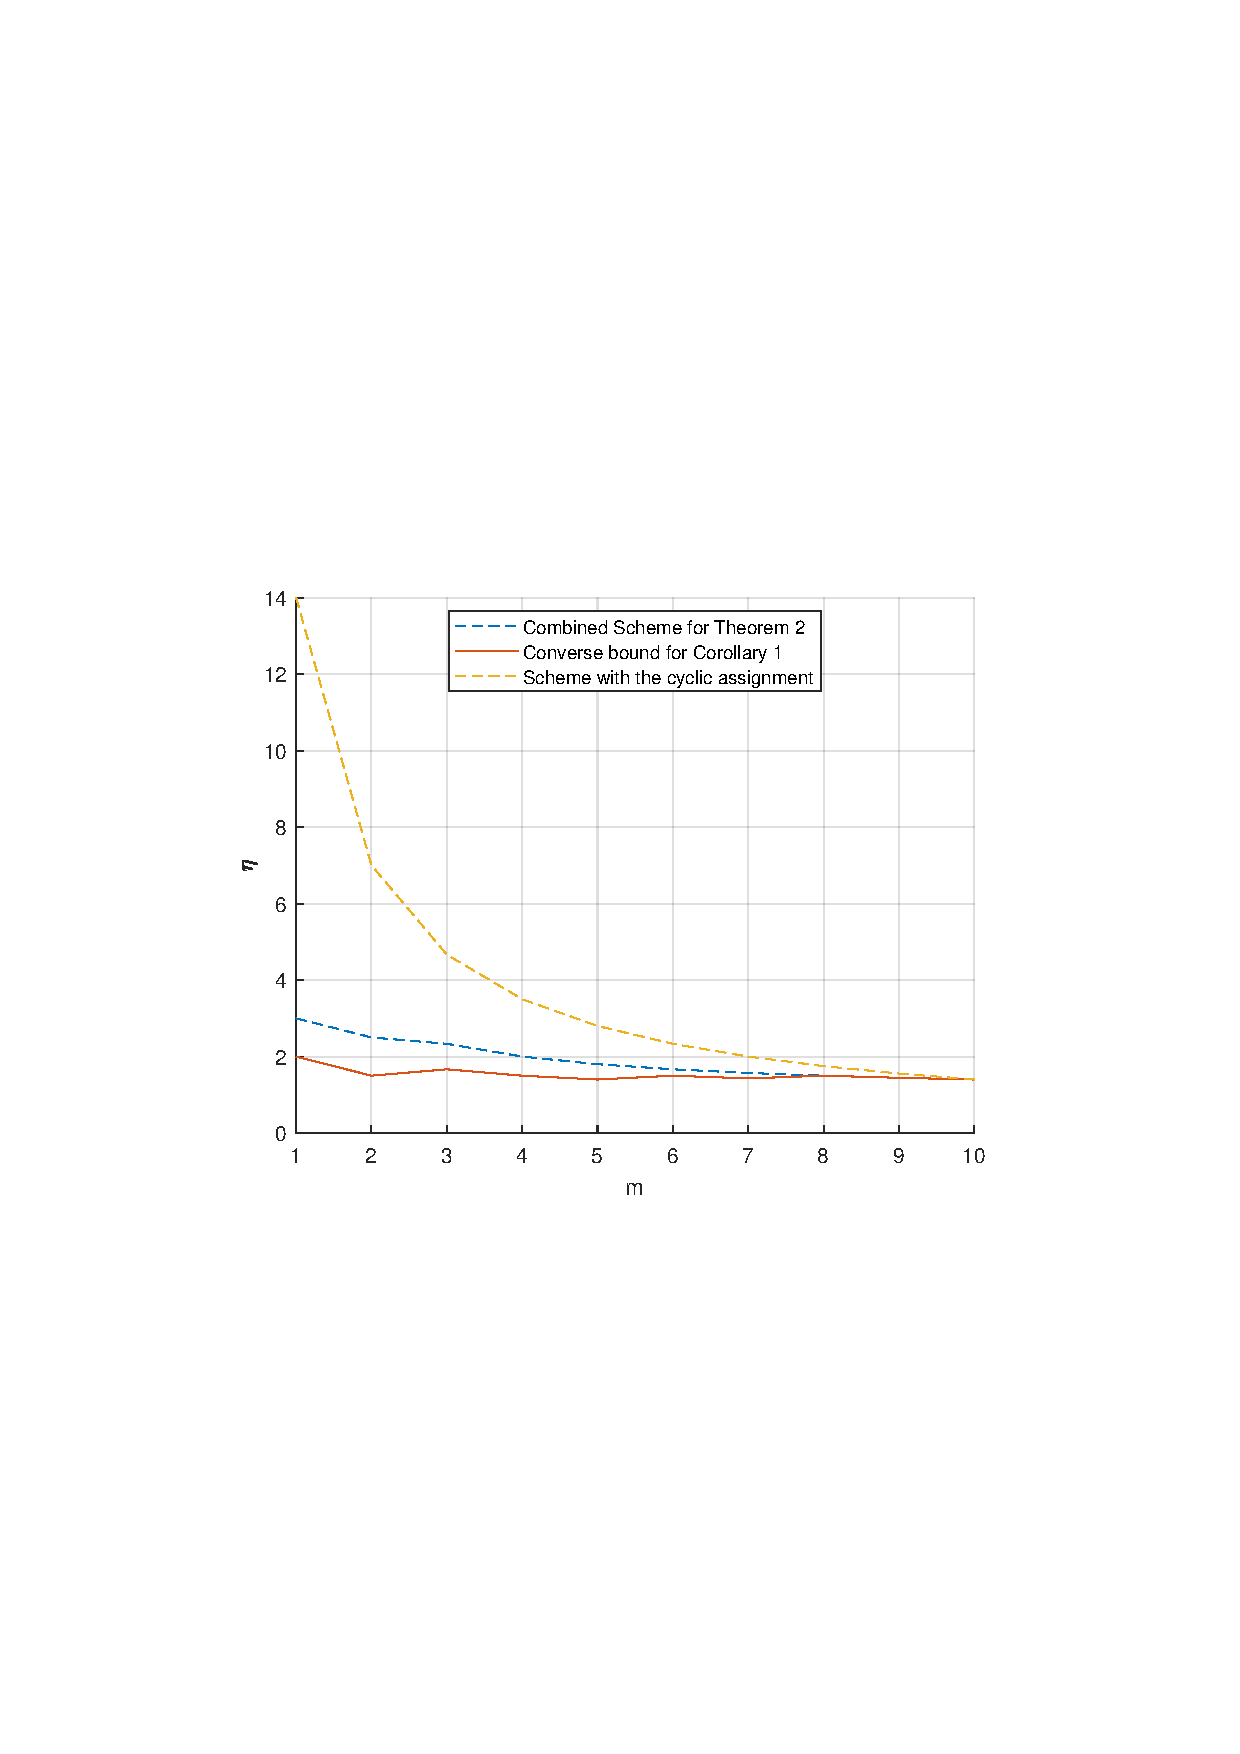
\includegraphics[scale=0.45]{m varies.pdf}
        \caption{\small $(\msf,\eta)$ tradeoff with $\Ksf = \Nsf=24, \Msf=10$.}
        \label{fig:numerical 1c}
    \end{subfigure}
    \caption{\small Numerical evaluations for the secure gradient coding .}
    \label{fig:numerical 1}
\end{figure}



\section{Novel Achievable Scheme For Theorem~\ref{thm:main achievable scheme}}
\label{sec:Achievable coding scheme}
\iffalse
Before presenting our scheme, we note that the $\Ksf$ datasets can be divided into $\Nsf$ non-overlapping groups, with the $i^{\text{th}}$ group $\Gc_i = \{k \in [\Ksf]: \text{Mod}(k,\Nsf) = i\}$ containing $\frac{\Ksf}{\Nsf}$ datasets. Each group $\Gc_i$ is assigned to $\Msf = \Nsf - \Nsf_{\rm r} + \msf$ servers, who collaboratively compute the merged message $W^{\prime}_i$. Thus, we reformulate the $(\Ksf, \Nsf, \Nsf_{\rm r}, 1, \Msf)$ secure distributed linearly separable computation problem as an equivalent $(\Nsf, \Nsf, \Nsf_{\rm r}, 1, \Msf)$ problem.
\fi
Recall Theorem~\ref{thm:bound of η}, which establishes that the key size is dependent on the data assignment. Due to space limitations, in the following, our analysis is confined to the case where $\Ksf = \Nsf$\footnote{Note that the $\Ksf$ datasets can be divided into $\Nsf$ non-overlapping groups, with the $i^{\text{th}}$ group $\Gc_i = \{k \in [\Ksf]: \text{Mod}(k,\Nsf) = i\}$ containing $\frac{\Ksf}{\Nsf}$ datasets. Each group $\Gc_i$ is assigned to $\Msf = \Nsf - \Nsf_{\rm r} + \msf$ servers, who collaboratively compute the merged message $W^{\prime}_i$. Thus, we reformulate the $(\Ksf, \Nsf, \Nsf_{\rm r}, 1, \Msf)$ secure distributed linearly separable computation problem as an equivalent $(\Nsf, \Nsf, \Nsf_{\rm r}, 1, \Msf)$ problem.}, with a particular focus on the data assignment. To elucidate the coding scheme, we present an illustrative example in Scheme~3. For a comprehensive treatment of the general scheme, readers are referred to Appendix~\ref{sec:general scheme}.

\subsection{\texorpdfstring{Scheme~1 for~\eqref{eq:from partial rep}}{Scheme 1 for Eq. (X)}}
\label{sub:partial rep}
In this section, we consider the case where $\Nsf > 2\Msf$. We partition servers and datasets into intervals of length \(\Msf\), i.e., \(\bigl[(i-1)\Msf + 1 : i\Msf\bigr]\) for \(i \in \Bigl[\Bigl\lfloor \frac{\Nsf}{\Msf} - 1 \Bigr\rfloor\Bigr]\), and assign them via the fractional repetition strategy, yielding \(\msf \Bigl\lfloor \frac{\Nsf}{\Msf} - 1 \Bigr\rfloor\) linearly independent combinations. We then assign the remaining \(\Nsf - \Bigl\lfloor \frac{\Nsf}{\Msf} - 1 \Bigr\rfloor \Msf\) datasets and servers, thereby reducing the original \((\Nsf, \Msf)\) problem to a smaller subproblem \(\bigl(\Nsf - \bigl\lfloor \tfrac{\Nsf}{\Msf} - 1 \bigr\rfloor \Msf, \Msf\bigr)\).


\iffalse
In conclusion, we have demonstrated that $h(\Nsf, \Msf) = \msf\left\lfloor \Nsf/\Msf - 1 \right\rfloor + h\left(\Nsf - \left\lfloor \Nsf/\Msf - 1 \right\rfloor \Msf, \Msf \right)$, which aligns with equation~\eqref{eq:from partial rep}. 
The detail of the proposed scheme is provided in Appendix~\ref{sec:general scheme}.
\fi
 
\subsection{\texorpdfstring{Scheme~2 for~\eqref{eq:M is even}}{Scheme 2 for Eq. (X)}}

\label{sub:M is even}

We consider the case \(1.5 \Msf \leq \Nsf < 2 \Msf\) with even \(\Msf \geq 2\msf\). The servers are divided into three groups: those in \([1, \tfrac{\Msf}{2}]\) (first group), those in \([\tfrac{\Msf}{2}+1, \Msf]\) (second group), and the remaining \(\Nsf - \Msf\) servers (third group). The first two groups each provide \(\msf\) linearly independent linear combinations, while the third group employs the \((\Nsf - \Msf, \tfrac{\Msf}{2})\) scheme to recover \(h(\Nsf - \Msf, \tfrac{\Msf}{2})\) combinations.



We first consider the data assignment for the servers in $[\Msf]$, whose structure is as follows.
\begin{align*}
\begin{array}{rl|c|c|c|c|c|c|c|}\cline{3-3}\cline{4-4}\cline{5-5}\cline{6-6}\cline{7-7}\cline{8-8}\cline{9-9}
&&\rule{0pt}{1.2em}\mbox{server}&\rule{0pt}{1.2em}\mbox{1} &\rule{0pt}{1.2em}\mbox{$\cdots$ } &  \rule{0pt}{1.2em}\mbox{ $\frac{\Msf}{2}$ } & \rule{0pt}{1.2em}\mbox{ $\frac{\Msf}{2}  +1$}&  \rule{0pt}{1.2em}\mbox{$\cdots$ } &  \rule{0pt}{1.2em}\mbox{$\Msf$ }\\ 
\cline{3-3}\cline{4-4}\cline{5-5}\cline{6-6}\cline{7-7}\cline{8-8}\cline{9-9}
&& &D_1 & \cdots & D_1 & D_1 & \cdots & D_1 \\
&& &\cdots & \cdots & \cdots & \cdots & \cdots & \cdots \\ 
&& \mbox{data}&D_{\ysf} & \cdots & D_{\ysf} & D_{\ysf} & \cdots & D_{\ysf} \\
&& &D_{\ysf+1} & \cdots & D_{\ysf+1} & D_{\Msf+1} & \cdots & D_{\Msf+1} \\ 
&& &\cdots & \cdots & \cdots & \cdots & \cdots & \cdots \\
&& &D_{\Msf} & \cdots & D_{\Msf}&  D_{\Nsf} & \cdots & D_{\Nsf}\\  
\cline{3-3}\cline{4-4}\cline{5-5}\cline{6-6}\cline{7-7}\cline{8-8}\cline{9-9}
\end{array}
\end{align*}


In this setup, we assign \(D_1\) to \(D_{\ysf}\) to all servers in \([\Msf]\), while each \(D_k\) for \(k \in [\ysf+1 : \Nsf]\) is assigned to \(\frac{\Msf}{2}\) servers in \([\Msf]\). We then allocate the remaining \(\Nsf-\Msf\) servers. Since \(\Nsf-\ysf = 2(\Nsf-\Msf)\) datasets (from \([\ysf+1 : \Nsf]\)) must be distributed among \(\Nsf-\Msf\) servers, each dataset is assigned to \(\frac{\Msf}{2}\) servers, and each server receives \(\Msf\) datasets. 

To implement this, we divide the datasets in \([\ysf+1 : \Nsf]\) into \(\frac{\Nsf-\ysf}{2} = \Nsf-\Msf\) pairs \(\Pc_i = \{\ysf + i, \Msf + i\}\) for \(i \in [\Nsf-\Msf]\). We then use the assignment phase of the \(\bigl(\Nsf-\Msf, \tfrac{\Msf}{2}\bigr)\) scheme, assigning each pair to \(\tfrac{\Msf}{2}\) servers, with each server receiving \(\tfrac{\Msf}{2}\) pairs.



\subsection{\texorpdfstring{Scheme~3 for~\eqref{eq:M is odd}}{Scheme 3 for Eq. (Y)}}
\label{sub:M is odd}
We provide an example to illustrate the main idea.
\begin{example} \rm
\label{ex:scheme 3 example}
We consider the $(\Nsf, \Msf) = (12, 7)$ non-secure problem, where $\msf = 2$.

{\it Data assignment phase.}
We assign the datasets as follows.  


\begin{align*}
\begin{array}{rl|c|c|c|}\cline{3-3}\cline{4-4}\cline{5-5}
&&\rule{0pt}{1.2em}\mbox{server}&\rule{0pt}{1.2em}\mbox{\textnormal{1}}  &\rule{0pt}{1.2em}\mbox{\textnormal{2}} \\ \cline{3-3}\cline{4-4}\cline{5-5}
&& &D_1 & D_1 \\
&& &D_2 & D_2  \\
&& &D_3 & D_3 \\
&& \mbox{data}&D_4 & D_4  \\
&& &D_5 & D_5 \\
&& &D_6 & D_6 \\
&& &D_7 & D_7\\
\cline{3-3}\cline{4-4}\cline{5-5}
\end{array}
\hspace{-0.5em} % 调整间隔大小
\begin{array}{rl|c|c|c|c|c|}\cline{3-3}\cline{4-4}\cline{5-5}\cline{6-6}\cline{7-7}
&&\rule{0pt}{1.2em}\mbox{\textnormal{3}} & \rule{0pt}{1.2em}\mbox{\textnormal{4}} & \rule{0pt}{1.2em}\mbox{\textnormal{5}} & \rule{0pt}{1.2em}\mbox{\textnormal{6}} & \rule{0pt}{1.2em}\mbox{\textnormal{7}} \\ \cline{3-3}\cline{4-4}\cline{5-5}\cline{6-6}\cline{7-7}
&&  D_1 & D_1 & D_1 & D_1 & D_1\\
&&   D_2 & D_2 & D_2 & D_2 & D_2 \\
&&  D_3 & D_3 & D_3 & D_3 & D_3\\
&&  D_8 & D_9 & D_{10} & D_{11} & D_{12} \\
&&  D_9 & D_{10} & D_{11} & D_{12} & D_8\\
&&  D_{10} & D_{11} & D_{12} & D_8 & D_9\\
&&  D_{11} & D_{12} & D_8 & D_9 & D_{10}\\
\cline{3-3}\cline{4-4}\cline{5-5}\cline{6-6}\cline{7-7}
\end{array}
\end{align*}


\begin{align*}
\begin{array}{rl|c|c|c|c|c|}\cline{3-3}\cline{4-4}\cline{5-5}\cline{6-6}\cline{7-7}
&&\rule{0pt}{1.2em}\mbox{\textnormal{8}} & \rule{0pt}{1.2em}\mbox{\textnormal{9}}  & \rule{0pt}{1.2em}\mbox{\textnormal{10}} & \rule{0pt}{1.2em}\mbox{\textnormal{11}} & \rule{0pt}{1.2em}\mbox{\textnormal{12}} \\ \cline{3-3}\cline{4-4}\cline{5-5}\cline{6-6}\cline{7-7}
&&  D_4& D_4 & D_4 & D_4 & D_4\\
&&  D_5& D_5 & D_5 & D_5 & D_5\\
&&  D_6& D_6 & D_6 & D_6 & D_6\\
&&  D_7& D_7 & D_7 & D_7 & D_7\\
&&  D_8& D_9 & D_{10} & D_{11} & D_{12}\\
&&  D_9& D_{10} & D_{11} & D_{12} & D_8\\
&&  D_{10}& D_{11} & D_{12} & D_8 & D_9 \\
\cline{3-3}\cline{4-4}\cline{5-5}\cline{6-6}\cline{7-7}
\end{array}
\end{align*}


{\it Computing phase.}
To minimize communication cost, each message $W_k$, for $k \in [\Ksf]$, is divided into $\msf$ equal-length sub-messages, denoted as $W_k = \{W_{k,j} : j \in [\msf]\}$, with each sub-message containing $\frac{\Lsf}{\msf} = \frac{\Lsf}{2}$ symbols in $\mathbb{F}_{\qsf}$. Each server sends a linear combination of messages, allowing the user to recover
\(\mathbf{F} [W_{1,1}; \ldots; W_{12,2}]\) from any \(\Nsf_{\rm r} = 7\) servers, where
\(\mathbf{F}\) (shown at the top of the next page in \eqref{eq:F of example3})
contains `$*$' symbols representing design variables.
We define that $[F_1;F_2;F_3;F_4;F_5;F_6]=  {\bf F} \  [W_{1,1};\ldots;W_{12,2}] $.
\begin{figure*}
\begin{equation}
 {\bf F} = \begin{bmatrix}  
 {\fv}_1 \\
 {\fv}_2 \\
 {\fv}_3 \\
 {\fv}_4\\
 {\fv}_5 \\
 {\fv}_6
 \end{bmatrix}
 =
 \left[
\begin{array}{cccccccccccccccccccccccc}
  1 & 1    &   1 &1 & 1  &     1 &1 & 1 &  1 & 1    &   1 &1 &   0 & 0  &0 &   0 & 0  &0 &   0 & 0  &0 &   0 & 0  &0     \\
   0 & 0  &0 &   0 & 0  &0 &   0 & 0  &0 &   0 & 0  &0  &  1 & 1    &   1 &1 & 1  &     1 &1 & 1 &  1 & 1    &   1 &1 \\
  0 & 0  &0  &  2 & 2 & 2  &2  &  1 &1 & 1  &1&1 &   0 & 0  &0  &   0 & 0  &0&   0 & 0  &0&   0 & 0  &0\\
  0 & 0  &0&   0 & 0  &0&   0 & 0  &0&   0 & 0  &0 & 0 & 0  &0  &  2 & 2 & 2  &2  &  1 &1 & 1  &1&1 \\
  0  & 0   &   0&0& 0   & 0  &0 &  * &* & *  &  * &*  &  0  & 0   &   0&0& 0   & 0  &0 &  * &* & *  &  * &* \\
   0  & 0   &   0&0& 0   & 0  &0 &  * &* & *  &  * &*  &  0  & 0   &   0&0& 0   & 0  &0 &  * &* & *  &  * &* \\
\end{array} 
\right]
 \label{eq:F of example3}
\end{equation} % 创建分割线
\end{figure*}

\textbf{We divide the servers into three groups based on the data assignment: servers 1 and 2 form the first group, those in $[3:7]$ form the second, and those in $[8:12]$ form the third. We require that the $\msf=2$ linear combinations \((F_1 - F_3)\) and \((F_2 - F_4)\) be recovered from the first group. From the second group, we recover \((2F_1 - F_3)\), \((2F_2 - F_4)\), \(F_5\), and \(F_6\), which together form \(\Nsf - \frac{3\Msf - 1}{2} + \msf = 4\) linear combinations, and from the third group, we recover \(F_3\), \(F_4\), \(F_5\), and \(F_6\), another \(4\) combinations. Hence, we can recover 
$\Nsf - \frac{3\Msf - 1}{2} + 2\msf = 6$ linear combinations in total, matching the result in~\eqref{eq:M is odd}. The following outlines the specific procedure.}



%In this case, the entries denoted by $*$ in the matrix cannot be simply chosen as random numbers, as in \cite{wan2022secure}. Instead, the values of $*$ need to be carefully constructed, and the specific reasons for this will be explained in the following details.

We focus on servers 1 and 2, which share the same datasets and exclude those from $[8{:}11]$. 
server~1 computes 
\[
X_1 = (F_1 - F_3) + (F_2 - F_4),
\]
and server~2 computes
\[
X_2 = (F_1 - F_3) - (F_2 - F_4).
\]
For servers handling $[8{:}12]$, we design transmissions so that $F_3, F_4, F_5,$ and $F_6$ 
can be recovered from any four responses. Specifically, for $n \in [8{:}12]$, let 
server~$n$ compute
\[
\sv_n \bigl[ \fv_3 ; \fv_4 ; \fv_5 ; \fv_6 \bigr] 
\bigl[ W_{1,1}; \ldots; W_{12,2} \bigr],
\]
where $\bigl[ \fv_3 ; \fv_4 ; \fv_5 ; \fv_6 \bigr]$ is given in 
\eqref{eq:scheme 3 transmission of second class} from Appendix~\ref{sec:general scheme}.



We design ${\bf s}_n$ according to the following steps. We focus on the datasets in $[8:12]$ under cyclic assignment, extracting the corresponding columns from the matrix to form a submatrix ${\bf F}^{\prime}_1$, where ${\bf F}^{\prime}_1$ is shown in \eqref{eq:scheme 3 sub transmission} from Appendix \ref{sec:general scheme}.
\iffalse
\begin{equation} \label{eq:scheme 3 sub transmission}
{\bf F}^{\prime}_1= \left[
\begin{array}{cccccccccc}
  1 & 1 & 1 & 1 & 1 & 0 & 0 & 0 & 0 & 0  \\
  0 & 0 & 0 & 0 & 0 & 1 & 1 & 1 & 1 & 1 \\
  * & * & * & * & * & * & * & * & * & * \\
  * & * & * & * & * & * & * & * & * & *
\end{array}
 \right].
\end{equation}
\fi
Notice that server $n$ cannot compute 2 of the datasets in $[8:12]$. We extract the corresponding columns from the matrix to form a submatrix $\overline{{\bf F}^{\prime}_1}$, where $\overline{{\bf F}^{\prime}_1}$ is shown in \eqref{eq:scheme 3 sub sub transmission} from Appendix \ref{sec:general scheme}.
\iffalse
where
\begin{equation} \label{eq:scheme 3 sub sub transmission}
\overline{{\bf F}^{\prime}_1}= \left[
\begin{array}{cccc}
  1 & 1 & 0 & 0  \\
  0 & 0 & 1 & 1 \\
  * & * & * & *  \\
  * & * & * & *
\end{array}
 \right].
\end{equation}
\fi
Our required ${\bf s}_n$ is the left null vector of $\overline{{\bf F}^{\prime}_1}$. 
\iffalse
If we choose the entries denoted by $*$ in ${\bf F}^{\prime}_1$ to be uniformly i.i.d. in $\mathbb{F}_q$ as in \cite{wan2022secure}, then $\overline{{\bf F}^{\prime}_1}$ will be full rank with high probability, meaning there will be no non-zero left null vector. Therefore, we employ the interference alignment strategy mentioned in \cite{limit} to construct $\overline{{\bf F}^{\prime}_1}$.
\fi

There should be a linear combination of the columns in $\overline{{\bf F}^{\prime}_1}$ leading to one rank deficiency, with the form
\begin{align}
 {\bf F}'_1 \ev_n^{\text{\rm T}} = {\bf 0}_{4 \times 1},
 \label{eq: linear reduction equation}
\end{align}
for the first row of $\overline{{\bf F}^{\prime}_1}$, since $\left[ {\begin{array}{cc} 1 & 1 \\ \end{array}} \right] [1, -1]^{\text{\rm T}} = {\bf 0}_{1 \times 1}$, the corresponding elements in $\ev_n$ should be a multiple of $(1, -1)$, and we choose a random multiple. Similarly, the same applies to the second row of $\overline{{\bf F}^{\prime}_1}$. Repeating the above steps, we obtain
\iffalse: 
\[
\ev_1 = (0, 0, 0, 1, -1, 0, 0, 0, -1, 1),
\]
\[
\ev_2 = (2, 0, 0, 0, -2, -1, 0, 0, 0, 1),
\]
\[
\ev_3 = (1, -1, 0, 0, 0, 2, -2, 0, 0, 0),
\]
\[
\ev_4 = (0, 1, -1, 0, 0, 0, 1, -1, 0, 0),
\]
\[
\ev_5 = (0, 0, -1, 1, 0, 0, 0, 2, -2, 0).
\]
These vectors form \fi
the matrix ${\bf E}$, where
\begin{align}
{\bf E} &= 
\left[ \ev_1 ;  \ev_2 ;  \ev_3 ;  \ev_4 ; \ev_5  \right] .
\label{eq:E for example}
\end{align}
The vector \(\ev_n\) is presented in Appendix~\ref{sec:general scheme}.

By \eqref{eq: linear reduction equation} and \eqref{eq:E for example}, we have
\begin{align}
{\bf F}'_1 {\bf E}^{\text{\rm T}} = \mathbf{0}_{4\times 5}, 
\label{eq:equations for example}
\end{align}

where ${\bf E}^{\text{\rm T}}$ is \(10 \times 5\) and full rank. Thus, its left null space contains \(5\) linearly independent vectors, spanning the rows of ${\bf F}'_1$. The first two rows lie in the null space of ${\bf E}^{\text{\rm T}}$, and any two vectors from the remaining three null space vectors complete ${\bf F}'_1$, given as:
\[
{\bf F}'_1 = 
\begin{bmatrix}
1 & 1 & 1 & 1 & 1 & 0 & 0 & 0 & 0 & 0 \\
0 & 0 & 0 & 0 & 0 & 1 & 1 & 1 & 1 & 1 \\
2 & 4 & 2 & 4 & 2 & 2 & 1 & 3 & 4 & 2 \\
2 & 2 & 4 & 4 & -2 & 3 & 3 & 1 & 1 & -5
\end{bmatrix}.
\]
For \({\bf s}_n\), satisfying \({\bf s}_n \overline{{\bf F}'_1} = \mathbf{0}_{1 \times 4}\), the resulting matrix is:
\[
{\bf S} = 
\begin{bmatrix}
{\bf s}_{1} \\
\vdots \\
{\bf s}_{5}
\end{bmatrix} =  
\begin{bmatrix}
 2 & 11/4 & -3/4 & 1/4 \\
 4 & 4 & -2 & 0 \\
 2 & 3 & 0 & -1 \\
 8 & 16/3 & -4/3 & -4/3 \\
 6 & 3/2 & 0 & -3/2 \\
\end{bmatrix}.
\]
For \(n \in [8, 12]\), server~\(n\) computes 
\[
X_n = {\bf s}_n \bigl[F_3; F_4; F_5; F_6\bigr].
\]

Next, servers in \([3{:}7]\), excluding datasets from \([4{:}7]\), ensure that responses from any \(4\) servers recover \((2F_1 - F_3)\), \((2F_2 - F_4)\), \(F_5\), and \(F_6\). For \(n \in [3, 7]\), server~\(n\) computes
\[
X_n = {\bf s}_n \bigl[2{\fv}_1 - {\fv}_3; 2{\fv}_2 - {\fv}_4; {\fv}_5; {\fv}_6\bigr]\bigl[W_{1,1}; \ldots; W_{12,2}\bigr],
\]
where \(\bigl[2{\fv}_1 - {\fv}_3; 2{\fv}_2 - {\fv}_4; {\fv}_5; {\fv}_6\bigr]\) is shown in \eqref{eq:scheme 3 transmission of first class} in Appendix~\ref{sec:general scheme}.

For datasets in \([8{:}12]\), cyclic assignment forms \({\bf F}'_2\), and it is evident that \({\bf F}'_2 = {\bf F}'_1\). Since datasets missing from server~\(n \in [3{:}7]\) are included in those missing from \(n+5\), we have \({\bf S}' = {\bf S}\). Thus, server~\(n\) computes
\[
X_n = {\bf s}_n \bigl[2F_1 - F_3; 2F_2 - F_4; F_5; F_6\bigr].
\]
 

Due to page limitations, we skip the proof of decodability. For more details, please refer to Appendix~\ref{sec:general scheme}.

In conclusion, under the condition $\msf = 2$, the number of totally transmitted linearly independent combinations is $h(12,7) = 12 - 10 + 4 = 6$, which coincides with~\eqref{eq:M is odd}.
\iffalse
{\it Decoding phase.}

From servers 1 and 2, the user can receive up to two linearly independent combinations. From the servers in $[3:7]$, the user can receive up to four linearly independent combinations, with any four of these five servers providing linearly independent combinations. Similarly, for the servers in $[8:12]$, the user can receive four linearly independent combinations from any four server responses.

The user receives responses from $N_{\rm r} = 12 - 7 + 2 = 7$ servers.
To recover $F_1$, $F_2$, $F_3$, $F_4$, $F_5$, and $F_6$, the user needs a total of six linearly independent combinations. We consider the following three cases:
\begin{itemize}
\item {\it Case 1: the user does not receive responses from servers 1 and 2.} In this case, the user will receive responses from any 7 servers in $[3:12]$. The worst case is when the user receives all responses from either the group $[3:7]$ or $[8:12]$, providing 4 linearly independent combinations, and responses from 2 servers in the other group, providing 2 additional linearly independent combinations. This totals 6 linearly independent combinations.

\item {\it Case 2: the user receives a response from either server 1 or 2.} Here, the user also receives responses from any 6 servers in $[3:12]$. The worst case is when all responses are received from one of the groups $[3:7]$ or $[8:12]$, providing 4 linearly independent combinations, along with a response from 1 server in the other group, contributing 1 additional linearly independent combination. This also totals 6 linearly independent combinations.

\item {\it Case 3: the user receives responses from both servers 1 and 2.} The user then receives responses from any 5 servers in $[3:12]$. In the worst case, the user receives all responses from either group $[3:7]$ or $[8:12]$, providing 4 linearly independent combinations. This again totals 6 linearly independent combinations.
\end{itemize}
It can be seen that under the condition $\msf = 2$, the number of totally transmitted linearly independent combinations is $h(12,7) = 12 - 10 + 4 = 6$, which coincides with~\eqref{eq:M is odd}.


\fi

\end{example}

\subsection{\texorpdfstring{Scheme~4 for~\eqref{eq:less than 1.5M}}{Scheme 4 for Eq. (Z)}}
\label{sub:less than 1.5M}
In this section, we consider the case \( \Msf < \Nsf < 1.5 \Msf \) with \( \Msf \ge 2 \msf \) and transform the \((\Nsf,\Msf)\) problem into \((\Msf, 2\Msf - \Nsf)\) by dividing the servers into two groups: those in \([\Msf]\) and those in \([\Msf+1 : \Nsf]\).
We assign \(D_1, \ldots, D_{\Nsf - \Msf}\) to each server in \([\Msf]\), and \(D_{\Nsf - \Msf + 1}, \ldots, D_{\Nsf}\) to each server in \([\Msf+1 : \Nsf]\). Thus, every server in \([\Msf+1 : \Nsf]\) holds \(\Msf\) datasets, while each server in \([\Msf]\) has \(\Nsf - \Msf\). Since every dataset in \([\Nsf - \Msf + 1 : \Nsf]\) is assigned to \(\Nsf - \Msf\) servers, we further assign each \(D_k\) (for \(k \in [\Nsf - \Msf + 1 : \Nsf]\)) to \(2\Msf - \Nsf\) additional servers in \([\Msf]\), giving each such server \((2\Msf - \Nsf)\) datasets. This allocation follows the assignment phase of the \((\Msf, 2\Msf - \Nsf)\) non-secure problem.


\iffalse
\section{Conclusion}
We focus on the secure distributed linearly separable computation problem, which prevents the user from accessing any information about the dataset besides the task function. We first research the minimum key size under general computation cost while achieving optimal communication cost. For this purpose, we propose a new computing scheme with a novel assignment strategy. The computing scheme can cover the optimality results of the computing scheme with fractional repetition assignment. The new computing scheme is also applicable to the case of minimal computation cost in \cite{wan2022secure}.
\fi

\clearpage
\bibliographystyle{IEEEtran}
\bibliography{re} 
\clearpage


  \appendices


\section{Proof of Theorem~\ref{thm:bound of η}}
\label{sec:bound proof}
By the security constraint in~\eqref{eq:security}, the user can only obtain $W_1+\cdots+W_{\Ksf}$ without accessing any additional information about the messages, even after receiving answers from all servers. Let $X_{\Sc}=\{X_n: n \in \Sc\}$. From~\eqref{eq:security}, we derive:
\begin{subequations}
\begin{align}
0 &= I(W_1, \ldots, W_{\Ksf}; X_{[\Nsf]} | W_1+W_2+\cdots+W_{\Ksf}) \\
  &= H(X_{[\Nsf]} | W_1+W_2+\cdots+W_{\Ksf}) - H(X_{[\Nsf]} | W_1, \ldots, W_{\Ksf}) \\
  &\geq H(X_{[\Nsf]} | W_1+W_2+\cdots+W_{\Ksf}) \nonumber\\
  &- H(Q, W_1, \ldots, W_{\Ksf} | W_1, \ldots, W_{\Ksf}) \label{eq:function of QW} \\
  &= H(X_{[\Nsf]} | W_1+W_2+\cdots+W_{\Ksf}) - H(Q) \label{eq:independent noise} \\
  &= H(X_{[\Nsf]}) - I(X_{[\Nsf]}; W_1+W_2+\cdots+W_{\Ksf}) - H(Q) \\
  &\geq H(X_{[\Nsf]}) - H(W_1+W_2+\cdots+W_{\Ksf}) - H(Q), \label{eq:shannon}
\end{align}
\end{subequations}
where~\eqref{eq:function of QW} follows from the fact that $X_{[\Nsf]}$ is a function of $Q$ and $W_1, \ldots, W_{\Ksf}$, and~\eqref{eq:independent noise} relies on $Q$ being independent of $W_1, \ldots, W_{\Ksf}$.

From~\eqref{eq:shannon}, we further obtain:
\begin{subequations}
\begin{align}
\eta \Lsf &\geq H(Q) \geq H(X_{[\Nsf]}) - H(W_1+\cdots+W_{\Ksf}) \\
          &\geq H(X_{[\Nsf]}) - \Lsf \label{eq:W1 inde} \\
          &\geq H(X_{s_1}, \ldots, X_{s_{|\sv|}}) - \Lsf \\
          &\geq  \frac{|\sv|\Lsf}{\msf} - \Lsf, \label{eq:lemma converse all term}
\end{align}
\end{subequations}
where~\eqref{eq:W1 inde} follows from the independence of $\Ksf$ messages, each uniformly i.i.d. over $[\mathbb{F}_{\qsf}]^{\Lsf}$. % and~\eqref{eq:lemma converse all term} is derived using the chain rule of entropy.

Prove of~\eqref{eq:lemma converse all term} Note that server $s_i$ always contains at least one message $W_{s_i}$ which can not be computed by $m$ servers from $\{s_1, \ldots, s_{i-1}\}$. Consider the case that apart from $\Nsf - \Nsf_{\rm r}$ stragglers, there are exactly $m$ servers who can compute $W_{s_i}$. Then,  the entropy of messages from these servers should be larger than $H(W_{s_i}) = \Lsf$. Without loss of generality, we assume $W_{s_i}$ can be computed by servers in $\{i,\ldots,\text{Mod}(i-m+1,|\sv|)\}$. We use \(\Wc\) to denote the set of messages excluding \(W_{s_1}, \ldots, W_{s_{|s|}}\) and use $\overline{W_{s_i}}$ to denote the set of all messages without $W_{s_i}$.
Consider the computation of messages $W_{s_1}, \ldots, W_{s_{|s|}}$, we have 
\begin{subequations}
\begin{align}
    &  mH(X_{s_1}, \ldots, X_{s_{|\sv|}}) \\
    & \geq m I(W_{s_1}, \ldots, W_{s_{|s|}};X_{s_1}, \ldots, X_{s_{|\sv|}} | \Wc) \\
    & = \sum_{n = 1}^{m} I(W_{s_n};X_{s_1}, \ldots, X_{s_{|\sv|}}| \Wc) + \ldots + \nonumber \\
     & \quad  I(W_{s_{\text{Mod} (n+|s|,|\sv|)}};X_{s_1}, \ldots, X_{s_{|\sv|}} \nonumber\\ & \quad | W_{s_n}, \ldots, W_{s_{\text{Mod}(n+|s|-1,|\sv|)}} , \Wc) \\
     & \geq \sum_{ i = 1}^{|\sv|} I(W_{s_i} ; X_{s_i},\ldots, X_{s_{\text{Mod}(i-m+1,|\sv|)}} | \overline{W_{s_{i}}} ) \\
     & \geq   |\sv| \Lsf.
\end{align}
\end{subequations}


\section{The general scheme of Theorem~\ref{thm:main achievable scheme}}
\label{sec:general scheme} 
\subsection{general scheme 1}
\label{general scheme 1}
{\it Data assignment phase.}
We partition the entire system into $\left\lfloor  \Nsf/\Msf \right\rfloor $ blocks. For each $i \in [\left\lfloor \Nsf/\Msf \right\rfloor - 1]$, the $i^{\text{th}}$ block includes the datasets $\{ D_{k}: k \in \left[(i-1)\Msf+1: i\Msf \right]\}$ and the servers in the range $\left[(i-1)\Msf+1: i\Msf \right]$.
The last block includes the datasets and servers in the range $\left[\left\lfloor \Nsf/\Msf - 1 \right\rfloor \Msf + 1 : \Nsf \right]$.

For the first $\left[\left\lfloor \Nsf/\Msf \right\rfloor - 1\right]$ blocks, we use the fractional repetition assignment to distribute the data. As for the last block, it contains $\Nsf - \left\lfloor \Nsf/\Msf - 1 \right\rfloor \Msf$ servers and $\Nsf - \left\lfloor \Nsf/\Msf - 1 \right\rfloor \Msf$ datasets, with each server being able to compute $M$ datasets. Therefore, we can directly apply the existing data assignment scheme designed for solving the $(\Nsf - \left\lfloor \Nsf/\Msf - 1 \right\rfloor \Msf, \Msf)$ non-secure problem to this last block.

{\it Computing phase.}
For each $i \in \left[\left\lfloor \Nsf/\Msf \right\rfloor - 1\right]$, each server in the $i^{\text{th}}$ block computes $m$ linear combinations $\sum_{k\in \left[(i-1)\Msf + 1 : i\Msf\right]} W_{k,j}$,  and each server sends a random linear combination of these $m$ computed combinations.

Next, we focus on the last block. The computation phase in this block still follows the $(\Nsf - \left\lfloor \Nsf/\Msf - 1 \right\rfloor \Msf, \Msf)$ non-secure scheme, which results in a total of $h\left(\Nsf - \left\lfloor \Nsf/\Msf - 1 \right\rfloor \Msf, \Msf\right)$ linearly independent combinations being sent.



{\it Decoding phase.}
The user receives information from $\Nsf_{\rm r} = \Nsf - \Msf + \msf$ servers, meaning that responses from $\Msf - \msf$ servers will not be received. For the first $\left\lfloor \Nsf/\Msf - 1 \right\rfloor$ blocks, each block has $\Msf$ servers, so at least $\msf$ servers' responses from each block are received by the user. Thus, from each block, the user can recover $\sum_{k \in \left[(i-1)\Msf + 1 : i\Msf\right]} W_{k,j}$, where $j$ ranges over $[\msf]$. 
For the last block, at least $\Nsf - \left\lfloor \Nsf/\Msf - 1 \right\rfloor \Msf - \Msf + \msf$ servers will respond. By carefully designing the coding scheme, we can recover $\sum_{k \in \left[\left\lfloor \Nsf/\Msf - 1 \right\rfloor \Msf + 1 : \Nsf\right]} W_k$ from the information sent by any $\Nsf - \left\lfloor \Nsf/\Msf - 1 \right\rfloor \Msf - \Msf + \msf$ servers in the last block.
together with the transmissions of the first $\left\lfloor  \Nsf/\Msf -1 \right\rfloor$ blocks, the user can recover $W_1 + \cdots +W_{\Nsf}$.

In conclusion, we have demonstrated that $h(\Nsf, \Msf) = \msf\left\lfloor \Nsf/\Msf - 1 \right\rfloor + h\left(\Nsf - \left\lfloor \Nsf/\Msf - 1 \right\rfloor \Msf, \Msf \right)$, which aligns with equation~\eqref{eq:from partial rep}. 
Furthermore, it is evident that $\Msf < \Nsf - \left\lfloor \Nsf/\Msf - 1 \right\rfloor \Msf < 2\Msf$ when $\Nsf > 2\Msf$ and $\Msf$ does not evenly divide $\Nsf$.

\subsection{general scheme 2}
\label{general scheme 2}
We now focus on the case where $1.5 \Msf \leq \Nsf < 2 \Msf$, and $\Msf$ is even, with $\Msf \geq 2\msf$. For this case, we consider the general Scheme 2 for the $(\Nsf, \Msf)$ non-secure problem to prove~\eqref{eq:M is even}. We assume that a specific feasible scheme already exists for the $\left(\Nsf - \Msf, \frac{\Msf}{2}\right)$ non-secure problem and that this scheme can transmit a total of $h\left(\Nsf - \Msf, \frac{\Msf}{2}\right)$ linearly independent combinations of messages.

{\it Data assignment phase.}
We first consider the dataset assignment for the servers in $[\Msf]$, which is structured as follows:
\begin{align*}
\begin{array}{rl|c|c|c|c|c|c|c|}\cline{3-3}\cline{4-4}\cline{5-5}\cline{6-6}\cline{7-7}\cline{8-8}\cline{9-9}
&&\rule{0pt}{1.2em}\mbox{server} & \rule{0pt}{1.2em}\mbox{1} &\rule{0pt}{1.2em}\mbox{$\cdots$ } &  \rule{0pt}{1.2em}\mbox{ $\frac{\Msf}{2}$ } & \rule{0pt}{1.2em}\mbox{ $\frac{\Msf}{2}  +1$}&  \rule{0pt}{1.2em}\mbox{$\cdots$ } &  \rule{0pt}{1.2em}\mbox{$\Msf$ }\\ 
\cline{3-3}\cline{4-4}\cline{5-5}\cline{6-6}\cline{7-7}\cline{8-8}\cline{9-9}
&& &D_1 & \cdots & D_1 & D_1 & \cdots & D_1 \\
&& &\cdots & \cdots & \cdots & \cdots & \cdots & \cdots \\ 
&& \mbox{data}&D_{\ysf} & \cdots & D_{\ysf} & D_{\ysf} & \cdots & D_{\ysf} \\
&& &D_{\ysf+1} & \cdots & D_{\ysf+1} & D_{\Msf+1} & \cdots & D_{\Msf+1} \\ 
&& &\cdots & \cdots & \cdots & \cdots & \cdots & \cdots \\
&& &D_{\Msf} & \cdots & D_{\Msf}&  D_{\Nsf} & \cdots & D_{\Nsf}\\  
\cline{3-3}\cline{4-4}\cline{5-5}\cline{6-6}\cline{7-7}\cline{8-8}\cline{9-9}
\end{array}
\end{align*}

In this setup, we assign datasets $D_1$ through $D_{\ysf}$ to all servers in $[\Msf]$, while each dataset $D_k$ for $k \in [\ysf+1 : \Nsf]$ is distributed among $\frac{\Msf}{2}$ servers in $[\Msf]$.

Next, we consider the assignment for the last $\Nsf-\Msf$ servers.
We need to allocate $\Nsf-\ysf = 2(\Nsf-\Msf)$ datasets (from $[\ysf+1 : \Nsf]$) to a total of $\Nsf-\Msf$ servers. Each dataset is assigned to $\frac{\Msf}{2}$ servers, and each server receives $\Msf$ datasets. 

Datasets in $[\ysf+1 : \Nsf]$ are divided into $\frac{\Nsf-\ysf}{2} = \Nsf-\Msf$ pairs, where the $i^{\text{th}}$ pair is defined as $\Pc_i = \{\ysf+i, \Msf+i\}$ for $i \in [\Nsf-\Msf]$. Thus, we apply the assignment phase of the scheme for the $\left(\Nsf-\Msf, \frac{\Msf}{2}\right)$ non-secure problem, assigning each pair to $\frac{\Msf}{2}$ servers, with each server being allocated $\frac{\Msf}{2}$ pairs.

{\it Computing phase.}
We divide each message $W_k$ for $k \in [\Ksf]$ into $\msf$ equal-length, non-overlapping sub-messages, denoted as $W_k = \{W_{k,j} : j \in [\msf]\}$.
We first focus on the servers in $[\Msf]$. By constructing the messages sent by these servers, we can recover the following $2\msf$ linear combinations:
\begin{align*}
    F_1 &= W_{1,1} + W_{2,1} + \cdots + W_{\Nsf,1}, \\
    &\vdots \\
    F_{\msf} &= W_{1,\msf} + W_{2,\msf} + \cdots + W_{\Nsf,\msf}, \\
    \\
    F_{\msf+1} &= 2(W_{\ysf+1,1} + \cdots + W_{\Msf,1}) + W_{\Msf+1,1} + \cdots + W_{\Nsf,1}, \\
    &\vdots \\
    F_{2\msf} &= 2(W_{\ysf+1,\msf} + \cdots + W_{\Msf,\msf}) + W_{\Msf+1,\msf} + \cdots + W_{\Nsf,\msf}.
\end{align*}

We group the $\msf$ linear combinations $(F_1 - F_{\msf+1}), \ldots, (F_{\msf} - F_{2\msf})$ into one group, and the $\msf$ linear combinations $(2F_1 - F_{\msf+1}), \ldots, (2F_{\msf} - F_{2\msf})$ into another group. Since the servers in $[\Msf/2]$ are not assigned any data from $[\Msf+1: \Nsf]$, we let each server in this range compute a random linear combination of the $\msf$ linear combinations in the first group. The servers in $[\Msf/2+1: \Msf]$, who are not assigned any data from $[\ysf+1: \Msf]$, are assigned to compute a random linear combination of the $\msf$ linear combinations in the second group.

We then focus on the servers in $[\Msf+1: \Nsf]$. For each dataset pair $\Pc_i = \{\ysf+i, \Msf+i\}$ where $i \in [\Nsf - \Msf]$, we define $P_i = 2W_{\ysf+i} + W_{\Msf+i}$. Therefore, we can express $F_{\msf+1}$ to $F_{2\msf}$ as $P_{1,1} + \cdots + P_{\Nsf-\Msf,1}, \ldots, P_{1,\msf} + \cdots + P_{\Nsf-\Msf,\msf}$.
Thus, we can apply the computing phase of the proposed scheme to the $\left(\Nsf - \Msf, \frac{\Msf}{2}\right)$ non-secure problem.

{\it Decoding phase.}

The user receives $\Nsf_{\rm r} = \Nsf - \Msf + \msf$ server responses, which can be categorized into two cases.

First, we consider the case where at least $\Nsf - 1.5\Msf + \msf$ responses come from servers in $[\Msf+1 : \Nsf]$. In this scenario, $F_{\msf+1}$ to $F_{2\msf}$ can be recovered. Additionally, at least $\msf$ responses from servers in $[\Msf]$ are received, providing at least $\msf$ linearly independent combinations. Together with the combinations from $F_{\msf+1}$ to $F_{2\msf}$, this gives a total of $2\msf$ linearly independent combinations, enabling recovery of $F_1$ to $F_{2\msf}$.
We then consider the second case, where the servers in $[\Msf+1: \Nsf]$ respond with $\Nsf - 1.5\Msf + \msf - \xsf$ responses, providing at least $h(\Nsf - \Msf, \Msf/2) - \xsf$ linearly independent combinations. Meanwhile, the servers in $[\Msf]$ will have $\Msf/2 + \xsf$ responses, contributing at least $\msf +\xsf$ linearly independent combinations. In total, these responses provide $h(\Nsf - \Msf, \Msf/2)$ linearly independent combinations, which are sufficient to recover $F_1$ to $F_{2\msf}$.

The number of linearly independent combinations transmitted by servers in $[\Msf+1:\Nsf]$ is $h\left(\Nsf-\Msf, \frac{\Msf}{2}\right)$, which spans the space containing $F_{\msf+1}$ to $F_{2\msf}$. Additionally, servers in $[\Msf]$ transmit $2\msf$ linearly independent combinations, also spanning the space of $F_{\msf+1}$ to $F_{2\msf}$. Therefore, the total number of transmitted linearly independent combinations is $h(\Nsf,\Msf)= 2\msf + h\left(\Nsf-\Msf, \frac{\Msf}{2}\right) - \msf = h\left(\Nsf-\Msf, \frac{\Msf}{2}\right) + \msf$, which matches~\eqref{eq:M is even}.

\subsection{general scheme 3}
\label{general scheme 3}

We first present the matrix omitted in Section~\ref{sub:M is odd}, given in 
~\ref{eq:scheme 3 sub transmission} and~\ref{eq:scheme 3 sub sub transmission}. 
At the top of the next page,~\ref{eq:scheme 3 transmission of second class} 
and~\ref{eq:scheme 3 transmission of first class} are shown.



\begin{equation} \label{eq:scheme 3 sub transmission}
{\bf F}^{\prime}_1= \left[
\begin{array}{cccccccccc}
  1 & 1 & 1 & 1 & 1 & 0 & 0 & 0 & 0 & 0  \\
  0 & 0 & 0 & 0 & 0 & 1 & 1 & 1 & 1 & 1 \\
  * & * & * & * & * & * & * & * & * & * \\
  * & * & * & * & * & * & * & * & * & *
\end{array}
 \right]
\end{equation}

\begin{equation} \label{eq:scheme 3 sub sub transmission}
\overline{{\bf F}^{\prime}_1}= \left[
\begin{array}{cccc}
  1 & 1 & 0 & 0  \\
  0 & 0 & 1 & 1 \\
  * & * & * & *  \\
  * & * & * & *
\end{array}
 \right]
\end{equation}

\[
\ev_1 = (0, 0, 0, 1, -1, 0, 0, 0, -1, 1),
\]
\[
\ev_2 = (2, 0, 0, 0, -2, -1, 0, 0, 0, 1),
\]
\[
\ev_3 = (1, -1, 0, 0, 0, 2, -2, 0, 0, 0),
\]
\[
\ev_4 = (0, 1, -1, 0, 0, 0, 1, -1, 0, 0),
\]
\[
\ev_5 = (0, 0, -1, 1, 0, 0, 0, 2, -2, 0).
\]
\begin{figure*}
\begin{equation} \label{eq:scheme 3 transmission of second class}
\begin{aligned}
\left[ {\fv}_3 ;  {\fv}_4 ;  {\fv}_5 ;  {\fv}_6 \right] = 
 \left[
\begin{array}{cccccccccccccccccccccccc}
 0 & 0 & 0 &  2 & 2 & 2 & 2 &  1 & 1 & 1 & 1 & 1 & 0 & 0 & 0 & 0 & 0 & 0 & 0 & 0 & 0 & 0 & 0 & 0 \\
 0 & 0 & 0 & 0 & 0 & 0 & 0 & 0 & 0 & 0 & 0 & 0 & 0 & 0 & 0 & 2 & 2 & 2 & 2 & 1 & 1 & 1 & 1 & 1 \\
 0 & 0 & 0 & 0 & 0 & 0 & 0 & * & * & * & * & * & 0 & 0 & 0 & 0 & 0 & 0 & 0 & * & * & * & * & * \\
 0 & 0 & 0 & 0 & 0 & 0 & 0 & * & * & * & * & * & 0 & 0 & 0 & 0 & 0 & 0 & 0 & * & * & * & * & *
\end{array}
 \right]
\end{aligned}
\end{equation}
\end{figure*}

\begin{figure*} [ht]
\begin{equation} \label{eq:scheme 3 transmission of first class}
\begin{aligned}
\begin{bmatrix}
 2{\fv}_1 - {\fv}_3 \\ 
 2{\fv}_2 - {\fv}_4 \\ 
 {\fv}_5 \\ 
 {\fv}_6 
\end{bmatrix} = 
 \left[
\begin{array}{cccccccccccccccccccccccc}
 2 & 2 & 2 & 0 & 0 & 0 & 0 & 1 & 1 & 1 & 1 & 1 & 0 & 0 & 0 & 0 & 0 & 0 & 0 & 0 & 0 & 0 & 0 & 0 \\
 0 & 0 & 0 & 0 & 0 & 0 & 0 & 0 & 0 & 0 & 0 & 0 & 2 & 2 & 2 & 0 & 0 & 0 & 0 & 1 & 1 & 1 & 1 & 1 \\
 0 & 0 & 0 & 0 & 0 & 0 & 0 & 2 & 4 & 2 & 4 & 2 & 0 & 0 & 0 & 0 & 0 & 0 & 0 & 2 & 1 & 3 & 4 & 2 \\
 0 & 0 & 0 & 0 & 0 & 0 & 0 & 2 & 2 & 4 & 4 & -2 & 0 & 0 & 0 & 0 & 0 & 0 & 0 & 3 & 3 & 1 & 1 & -5
\end{array}
 \right].
\end{aligned}
\end{equation}

\end{figure*}

We now consider the $(\Nsf, \Msf)$ non-secure problem, where $1.5 \Msf \leq \Nsf < 2\Msf$, $\Msf$ is odd, and $\Msf \geq 2\msf + 1$. Our goal is to construct a scheme (Scheme~3) to prove~\eqref{eq:M is odd}.
We also define that $\Nsf=2\Msf-\ysf$. 

{\it Data assignment phase.}
The assignment is shown at the top of the next page.
\begin{figure*}
\begin{align*}
\begin{array}{rl|c|c|c|c|c|c|c|c|c|c|c|c|}\cline{3-3}\cline{4-4}\cline{5-5}\cline{6-6}\cline{7-7}\cline{8-8}\cline{9-9}\cline{10-10}\cline{11-11}\cline{12-12}\cline{13-13}\cline{14-14}
&&\rule{0pt}{1.2em}\mbox{\small server} &\rule{0pt}{1.2em}\mbox{\small \negmedspace\negmedspace 1 \negmedspace\negmedspace} & \mbox{\small \negmedspace\negmedspace $\cdots$ \negmedspace\negmedspace} &  \rule{0pt}{1.2em}\mbox{\small \negmedspace\negmedspace $\ysf$ \negmedspace\negmedspace}& \rule{0pt}{1.2em}\mbox{\small \negmedspace\negmedspace  $\ysf +1$ \negmedspace\negmedspace}&  \rule{0pt}{1.2em}\mbox{\small \negmedspace\negmedspace  $\ysf+2$ \negmedspace\negmedspace}&  \rule{0pt}{1.2em}\mbox{\small \negmedspace\negmedspace $\cdots$ \negmedspace\negmedspace} &  \rule{0pt}{1.2em}\mbox{\small \negmedspace\negmedspace $\Msf$ \negmedspace\negmedspace} &\rule{0pt}{1.2em}\mbox{\small \negmedspace\negmedspace  $\Msf$+1 \negmedspace\negmedspace} & \rule{0pt}{1.2em}\mbox{\small \negmedspace\negmedspace  $\Msf+2$ \negmedspace\negmedspace} & \rule{0pt}{1.2em}\mbox{\small \negmedspace\negmedspace $\cdots$\negmedspace\negmedspace }& \rule{0pt}{1.2em}\mbox{\small \negmedspace\negmedspace $\Nsf$\negmedspace\negmedspace} \\ 
\cline{3-3}\cline{4-4}\cline{5-5}\cline{6-6}\cline{7-7}\cline{8-8}\cline{9-9}\cline{10-10}\cline{11-11}\cline{12-12}\cline{13-13}\cline{14-14}
&& &D_1& \cdots       &   D_1 &  D_{1} &  D_{1} & \cdots &  D_{1}   &  D_{\frac{\Msf-1}{2}+1}   &  D_{\frac{\Msf-1}{2}+1} &  \cdots  &  D_{\frac{\Msf-1}{2}+1}  \\
&& &\cdots & \cdots & \cdots &  \cdots & \cdots  & \cdots   & \cdots  & \cdots & \cdots & \cdots & \cdots  \\ 
&& \mbox{\small data}&D_{\frac{\Msf-1}{2}} &    \cdots    & D_{\frac{\Msf-1}{2}}  & D_{\frac{\Msf-1}{2}} & D_{\frac{\Msf-1}{2}}    & \cdots  & D_{\frac{\Msf-1}{2}} &   D_{\Msf}  &   D_{\Msf}  &  \cdots  &  D_{\Msf}  \\
&& &D_{\frac{\Msf-1}{2}+1}&  \cdots  & D_{\frac{\Msf-1}{2}+1}  & D_{\Msf+1} & D_{\Msf+2} & \cdots & D_{\Nsf}& D_{\Msf+1}  &  D_{\Msf+2} &   \cdots  &  D_{\Nsf} \\ 
&& &\cdots &  \cdots       & \cdots & \cdots & \cdots   & \cdots & \cdots & \cdots & \cdots   & \cdots & \cdots \\
&& &D_{\Msf} &   \cdots  &  D_{\Msf} & D_{\frac{3\Msf+1}{2}} & D_{\frac{3\Msf+1}{2} +1}  & \cdots & D_{\frac{\Msf+1}{2}-1} &  D_{\frac{3\Msf-1}{2}}  &  D_{\frac{3\Msf-1}{2}+1}   &  \cdots  &  D_{\frac{\Msf-1}{2}-1}\\  
\cline{3-3}\cline{4-4}\cline{5-5}\cline{6-6}\cline{7-7}\cline{8-8}\cline{9-9}\cline{10-10}\cline{11-11}\cline{12-12}\cline{13-13}\cline{14-14}
\end{array} 
\end{align*}
\end{figure*}
In this assignment, we split the $\Nsf$ datasets into three sections. The first section includes $D_1, \ldots, D_t$ (The reason for choosing $t = \frac{\Msf - 1}{2}$ is provided in \cite{wan2022secure}.), and these datasets are assigned to servers in $[\Msf]$. The second section, containing $D_{t+1}, \ldots, D_{\Msf}$, is assigned to servers in $[\ysf] \cup [\Msf+1 : \Nsf]$. The third section, consisting of $D_{\Msf+1}, \ldots, D_{\Nsf}$, is cyclically allocated to servers in $[\ysf+1 : \Msf]$, where each server receives $\Msf - t$ adjacent datasets within $\left[{\frac{\Msf - 1}{2} + 1} : \Nsf \right]$. Additionally, datasets $D_{\Msf+1}, \ldots, D_{\Nsf}$ are assigned to servers in $[\Msf+1 : \Nsf]$ in a cyclic manner such that each server receives $t$ consecutive datasets within $\left[{\frac{\Msf - 1}{2} + 1} : \Nsf \right]$.

  {\it Computing phase.}
  We first divide each message $W_k$ for $k \in [\Ksf]$ into $\msf$ equal-length, non-overlapping sub-messages, denoted as $W_k = \{W_{k,j} : j \in [\msf]\}$.
We design the computing phase so that the total number of linearly independent combinations computed by all servers is $\ \frac {\Msf + 1}{2} - \ysf + 2\msf$. We let each server send a linear combination of messages so that the user can recover ${\bf F}' \ [W_{1,1}; \ldots; W_{\Nsf,\msf}]$ from the responses of any $N_{\rm r} = \Nsf - \Msf +\msf$ servers, where \( {\bf F}' \) is shown at the top of the next page in \eqref{eq:general form of F'}.
\begin{figure*}
\begin{equation}
 {\bf F}' = \begin{bmatrix}
 \fv_1 \\
 \vdots \\
 \fv_{\frac{\Msf+1}{2}-\ysf+2\msf} 
 \end{bmatrix}
 =
\left[
\begin{array}{c:c:c:c}
 ({\bf F})_{2 \times \Nsf}  & {\bf 0}_{2 \times \Nsf}  & \cdots & {\bf 0}_{2 \times \Nsf}   \\ \hdashline
{\bf 0}_{2 \times \Nsf} &  ({\bf F})_{2 \times \Nsf}   & \cdots & {\bf 0}_{2 \times \Nsf}   \\ \hdashline 
 \vdots   & \vdots  &  \ddots & \vdots \\ \hdashline
 {\bf 0}_{2 \times \Nsf} &   {\bf 0}_{2 \times \Nsf}    & \cdots &  ({\bf F})_{2 \times \Nsf} \\ \hdashline
 ({\bf V}_{1})_{ (\frac{\Msf + 1}{2} - \ysf) \times \Nsf}  &  ({\bf V}_{2})_{ (\frac{\Msf + 1}{2} - \ysf) \times \Nsf}  &   \cdots   &   ({\bf V}_{\msf})_{ (\frac{\Msf + 1}{2} - \ysf) \times \Nsf} 
 \end{array}
\right]_{(\frac{\Msf + 1}{2} - \ysf + 2\msf) \times \Nsf\msf}.
\label{eq:general form of F'}
\end{equation}
\rule{\textwidth}{0.2pt} % 创建分割线
\end{figure*}

We design the demand matrix 
\begin{equation}
\bf F = 
\begin{bmatrix}
\tikzmark{left4F} \textcolor{white}{0} 1 , \ldots , 1 \textcolor{white}{0} \tikzmark{right4F} & 
\tikzmark{left5F} \textcolor{white}{0} 1 , \ldots , 1 \textcolor{white}{0} \tikzmark{right5F} & 
\tikzmark{left6F} \textcolor{white}{0} 1 , \ldots , 1 \textcolor{white}{0} \tikzmark{right6F} \\
\textcolor{white}{0} 0 , \ldots , 0 \textcolor{white}{0} & 
\textcolor{white}{0} 2 , \ldots , 2 \textcolor{white}{0} & 
\textcolor{white}{0} 1 , \ldots , 1 \textcolor{white}{0} 
\end{bmatrix}
\label{eq: general of F}
\end{equation}

\DrawboxF[thick, black, dashed]{left4F}{right4F}{\textcolor{black}{\footnotesize${\bf C}_1$}}
\DrawboxF[thick, red, dashed]{left5F}{right5F}{\textcolor{red}{\footnotesize${\bf C}_2$}}
\DrawboxF[thick, blue, dashed]{left6F}{right6F}{\textcolor{blue}{\footnotesize${\bf C}_3$}}\\


We divide matrix ${\bf F}$ into three column-wise sub-matrices: ${\bf C}_1$, containing $\frac{\Msf-1}{2}$ columns, corresponding to the messages in $\left[\frac{\Msf-1}{2} \right]$, ${\bf C}_2$, containing $\frac{\Msf+1}{2}$ columns, corresponding to the messages in $\left[\frac{\Msf+1}{2} : \Msf \right]$, and ${\bf C}_3$, containing $(\Nsf - \Msf)$ columns, corresponding to the messages in $[\Msf+1 : \Nsf]$.


Let the matrix ${\bf V}_i$, for $i \in [\msf]$, be defined as
\begin{equation}
{\bf V}_i = 
\begin{bmatrix}
\tikzmark{left4V} \textcolor{white}{0} 0 , \ldots , 0 \textcolor{white}{0} \tikzmark{right4V} & 
\tikzmark{left5V} \textcolor{white}{0} 0 , \ldots , 0 \textcolor{white}{0} \tikzmark{right5V} & 
\tikzmark{left6V} \textcolor{white}{0} * , \ldots , * \textcolor{white}{0} \tikzmark{right6V} \\
\vdots & \vdots & \vdots \\
\textcolor{white}{0} 0 , \ldots , 0 \textcolor{white}{0} & 
\textcolor{white}{0} 0 , \ldots , 0 \textcolor{white}{0} & 
\textcolor{white}{0} * , \ldots , * \textcolor{white}{0} 
\end{bmatrix}
\label{eq:general form of V_i}
\end{equation}

% Draw dashed boxes with labels for each column to include all rows
\DrawboxV[thick, black, dashed]{left4V}{right4V}{\textcolor{black}{\footnotesize${\bf C}_1$}}
\DrawboxV[thick, red, dashed]{left5V}{right5V}{\textcolor{red}{\footnotesize${\bf C}_2$}}
\DrawboxV[thick, blue, dashed]{left6V}{right6V}{\textcolor{blue}{\footnotesize${\bf C}_3$}}

In the matrix ${\bf V}_i$, the entries denoted by $*$ are the unknowns that we need to design. And ${\bf C}_1$, ${\bf C}_2$, and ${\bf C}_3$ have column counts consistent with the definitions above.

Now, we focus on the servers in $[\ysf]$, which have the same datasets and do not contain datasets from $[\Msf+1 : \Nsf]$. From these servers, we aim to recover:
\begin{align*}
    F_1 - F_2 &= W_{1,1} + \cdots + W_{t,1} - W_{t+1,1} - \cdots - W_{\Nsf,1}, \\
    &\vdots \\
    F_{2\msf - 1} - F_{2\msf} &= W_{1,\msf} + \cdots + W_{t,\msf} - W_{t+1,\msf} - \cdots - W_{\Nsf,\msf}.
\end{align*}
Thus, we let the servers in $[\ysf]$ each compute a random linear combination of the $m$ linearly independent combinations $(F_1 - F_2), \ldots, (F_{2\msf - 1} - F_{2\msf})$.

For the servers in $[M+1 : N]$ that do not contain datasets from $[t]$, we design their transmissions so that the user can recover $F_2, F_4, \ldots, F_{2\msf}, F_{2\msf+1}, \ldots, F_{\frac{\Msf+1}{2} - \ysf + 2\msf}$ from any $\frac{\Msf+1}{2} - \ysf + \msf$ responses.
 For $n \in [\Msf+1, \Nsf]$, we let server $n$ compute
\begin{align}
{\bf s}_n  & [ F_2; F_4; \ldots; F_{2\msf}; F_{2\msf+1}; \ldots; F_{\frac{\Msf+1}{2} - \ysf + 2\msf} ]  \nonumber \\
& \text{× }  [ W_{1,1}; W_{2,1}; \ldots; W_{\Nsf,\msf} ] .
\label{eq:transmission of second class}
\end{align}
We design ${\bf s}_{n} $ as follows.
Notice that $W_1, \ldots, W_{\frac{\Msf-1}{2}}$ can be computed by server $n$; and that in the linear combination~\eqref{eq:transmission of second class}, the coefficients of $W_{\frac{\Msf-1}{2}+1}, \ldots, W_{\Msf}$ are $0$. 
Hence, in order to guarantee that in~\eqref{eq:transmission of second class} the coefficients of the messages which server $n$ cannot compute are $0$, we only need to consider the messages in $W_{\Msf+1}, \ldots, W_{\Nsf}$, corresponding to the columns in ${\bf C}_3$ in the matrix, with a total of $\msf (\Nsf - \Msf)$ columns.
By extracting the corresponding rows and columns from the matrix \( {\bf F}' \), we obtain \( {\bf F}_{\bf s} \), as shown at the top of the next page in \eqref{eq:general form of F_s},
\begin{figure*}
\begin{equation}
 {\bf F}_{\bf s} = 
\left[
\begin{array}{c:c:c:c}
{\bf 1}_{1 \times (\Nsf-\Msf)}  & {\bf 0}_{1 \times (\Nsf-\Msf)}  & \cdots & {\bf 0}_{1 \times (\Nsf-\Msf)}   \\ \hdashline
{\bf 0}_{1 \times (\Nsf-\Msf)} &  {\bf 1}_{1 \times (\Nsf-\Msf)}   & \cdots & {\bf 0}_{1 \times (\Nsf-\Msf)}   \\ \hdashline 
 \vdots   & \vdots  &  \ddots & \vdots \\ \hdashline
 {\bf 0}_{1 \times (\Nsf-\Msf)} &   {\bf 0}_{1 \times (\Nsf-\Msf)}    & \cdots &  {\bf 1}_{1 \times (\Nsf-\Msf)} \\ \hdashline
 ({\bf V}'_{1})_{ (\frac{\Msf + 1}{2} - \ysf) \times (\Nsf-\Msf)}  &  ({\bf V}'_{2})_{ (\frac{\Msf + 1}{2} - \ysf) \times (\Nsf-\Msf)}  &   \cdots   &   ({\bf V}'_{\msf})_{ (\frac{\Msf + 1}{2} - \ysf) \times (\Nsf-\Msf)} 
 \end{array}
\right]_{(\frac{\Msf + 1}{2} - \ysf + \msf) \times \msf(\Nsf-\Msf)}
\label{eq:general form of F_s}
\end{equation}

\end{figure*}
where ${\bf V}'_i$ is the sub-matrix formed by the last $\Nsf - \Msf$ columns of ${\bf V}_i$.
Notice that the datasets in $[\Msf+1 : \Nsf]$ are placed in a cyclic assignment among the servers in $[\Msf+1 : \Nsf]$. Each server cannot compute $\Nsf - \Msf - \frac{\Msf - 1}{2}$ of the datasets in $[\Msf+1 : \Nsf]$. By extracting the corresponding columns from the matrix ${\bf F}_{\bf s}$, we form a submatrix ${\bf F}_{{\bf s}_n}$, with dimensions 
$\left(\frac{\Msf + 1}{2} - \ysf + \msf\right) \times \msf \left(\Nsf - \frac{3\Msf - 1}{2}\right)$.
Our desired vector ${\bf s}_n$ is then the left null vector of this matrix.
If the number of rows in the matrix ${\bf F}_{{\bf s}_n}$ is greater than the number of columns, we can directly assign random values to the entries denoted by $*$ as in \cite{wan2022secure} to obtain ${\bf s}_n$. If the number of rows is less than or equal to the number of columns, we apply the interference alignment strategy from \cite{limit} to design the values of the $*$ entries in order to obtain ${\bf s}_n$.

Finally, we focus on the servers in $[\ysf+1 : \Msf]$. We design their transmissions so that the user can recover $2F_1 - F_2, 2F_3 - F_4, \ldots, 2F_{2\msf-1} - F_{2\msf}, F_{2\msf+1}, \ldots, F_{\frac{\Msf+1}{2} - \ysf + 2\msf}$ from any $\frac{\Msf+1}{2} - \ysf + \msf$ responses.
 For $n \in [\ysf+1, \Msf]$, we also let server $n$ compute
\begin{align}
{\bf s}_n & [ 2F_1 - F_2; \ldots; 2F_{2\msf-1} - F_{2\msf}; F_{2\msf+1}; \ldots; F_{\frac{\Msf+1}{2} - \ysf + 2\msf} ]  \nonumber \\
& \text{× }[ W_{1,1}; W_{2,1}; \ldots; W_{\Nsf,\msf} ].
\label{eq:transmission of first class}
\end{align}
     We design ${\bf s}_{n} $ as follows.
Notice that $W_1,\ldots,W_{\frac{\Msf-1}{2}}$ can be computed by server $n$; and that in the linear combination~\eqref{eq:transmission of first class} the coefficients of   $W_{\frac{\Msf-1}{2}+1}, \ldots, W_{\Msf}$ are $0$. 
Hence, in order to guarantee that in~\eqref{eq:transmission of first class} the coefficients of the messages which server $n$ cannot compute are $0$, we only need to consider the messages in $W_{\Msf+1}, \ldots, W_{\Nsf}$,corresponding to the columns in ${\bf C}_3$ in the matrix, with a total of $\msf (\Nsf - \Msf)$ columns.By extracting the corresponding rows and columns from the matrix \( {\bf F}' \), we obtain \( {\bf F}'_{\bf s} \), as shown at the top of the next page in \eqref{eq:general form of F'_s}.
\begin{figure*}
\begin{equation}
 {\bf F}'_{\bf s} = 
\left[
\begin{array}{c:c:c:c}
{\bf 1}_{1 \times (\Nsf-\Msf)}  & {\bf 0}_{1 \times (\Nsf-\Msf)}  & \cdots & {\bf 0}_{1 \times (\Nsf-\Msf)}   \\ \hdashline
{\bf 0}_{1 \times (\Nsf-\Msf)} &  {\bf 1}_{1 \times (\Nsf-\Msf)}   & \cdots & {\bf 0}_{1 \times (\Nsf-\Msf)}   \\ \hdashline 
 \vdots   & \vdots  &  \ddots & \vdots \\ \hdashline
 {\bf 0}_{1 \times (\Nsf-\Msf)} &   {\bf 0}_{1 \times (\Nsf-\Msf)}    & \cdots &  {\bf 1}_{1 \times (\Nsf-\Msf)} \\ \hdashline
 ({\bf V}'_{1})_{ (\frac{\Msf + 1}{2} - \ysf) \times (\Nsf-\Msf)}  &  ({\bf V}'_{2})_{ (\frac{\Msf + 1}{2} - \ysf) \times (\Nsf-\Msf)}  &   \cdots   &   ({\bf V}'_{\msf})_{ (\frac{\Msf + 1}{2} - \ysf) \times (\Nsf-\Msf)} 
 \end{array}
\right]_{(\frac{\Msf + 1}{2} - \ysf + \msf) \times \msf(\Nsf-\Msf)}.
\label{eq:general form of F'_s}
\end{equation}
\rule{\textwidth}{0.2pt} % 创建分割线
\end{figure*}
It is easy to observe that ${\bf F}'_{\bf s} = {\bf F}_{\bf s}$.Notice that the datasets in $[\Msf+1, \Nsf]$ are also cyclically assigned to the servers in $[\ysf+1 : \Msf]$. For $n \in [\ysf+1 : \Msf]$, server $n$ cannot compute ${\Nsf - \frac{3\Msf + 1}{2}}$ datasets from $[\Msf+1, \Nsf]$, and these datasets are also not computable by server $n + \Msf - \ysf$. Since ${\bf F}'_{\bf s} = {\bf F}_{\bf s}$, we can  set ${\bf s}_n = {\bf s}_{n + \Msf - \ysf}$.

  
  {\it Decoding phase.}
The user receives responses from $N_{\rm r} = \Nsf - \Msf + \msf$ servers, of which $x$ responses are from servers in $[\ysf]$. Depending on the value of $\xsf$, we can categorize the scenarios into the following two cases:
\begin{itemize}
\item {\it Case 1: $\xsf \leq \msf$.} In this case, the user receives $\xsf$ linearly independent combinations sent by the servers in $[\ysf]$. The user still needs to collect an additional $2\msf - \xsf + \Nsf - \frac{3\Msf - 1}{2}$ linearly independent combinations from any $(\Nsf - \Msf - \xsf + \msf)$ servers in $[\ysf + 1 : \Nsf]$.
In the worst-case scenario, the servers in one of the groups, either $[\ysf + 1 : \Msf]$ or $[\Msf + 1 : \Nsf]$, all respond, transmitting a total of $\msf + \Nsf - \frac{3\Msf - 1}{2}$ linearly independent combinations. Additionally, $\msf - \xsf$ servers from the other group respond, providing another $\msf - \xsf$ linearly independent combinations. 

Together, this results in a total of $2\msf + \Nsf - \frac{3\Msf - 1}{2}$ linearly independent combinations, sufficient to fully recover the demand matrix ${\bf F}'$.

\item {\it Case 2: $\msf < \xsf \leq \ysf$.} In this case, the user receives $\msf$ linearly independent combinations sent by the servers in $[\ysf]$. We consider the worst-case scenario, where $x = \ysf$, meaning that the user still needs to collect an additional $\msf + \Nsf - \frac{3\Msf - 1}{2}$ linearly independent combinations from any $2\Nsf - 3\Msf + \msf$ servers in $[\ysf + 1 : \Nsf]$.
Since $\Nsf \geq \frac{3\Msf + 1}{2}$, it follows that $2\Nsf - 3\Msf + \msf \geq \msf + \Nsf - \frac{3\Msf - 1}{2}$. Additionally, any $\msf + \Nsf - \frac{3\Msf - 1}{2}$ servers in either of the groups $[\ysf + 1 : \Msf]$ or $[\Msf + 1 : \Nsf]$ compute linearly independent combinations. Therefore, it is possible to receive $\msf + \Nsf - \frac{3\Msf - 1}{2}$ linearly independent combinations from any $2\Nsf - 3\Msf + \msf$ servers in $[\ysf + 1 : \Nsf]$.
\end{itemize}
Thus, the user obtains a total of $2\msf + \Nsf - \frac{3\Msf - 1}{2}$ linearly independent combinations, which suffices to reconstruct the demand matrix ${\bf F}'$.

 By the above scheme,  the number of linearly independent transmissions by all servers is equal to the number of rows in ${\bf F}'$, i.e.,
$\frac{\Msf+1}{2}-\ysf+2\msf =\Nsf- \frac{3\Msf-1}{2}+2\msf $, coinciding with~\eqref{eq:M is odd}.

\subsection{general scheme 4}
\label{general scheme 4}
In this section, we examine the case where $\Msf < \Nsf < 1.5 \Msf$, with $\Msf \geq 2\msf$, and construct a recursive scheme (Scheme~4) that aims to demonstrate~\eqref{eq:less than 1.5M}. This recursive scheme builds on the solution for the $(\Msf, 2\Msf-\Nsf)$ non-secure problem, assuming that this solution has been previously developed, and provides a total of $h(\Msf, 2\Msf-\Nsf)$ linearly independent combinations of messages.

{\it Data assignment phase.} We begin by allocating datasets $D_{1}, \ldots, D_{\Nsf-\Msf}$ to each server in $[\Msf]$. Subsequently, datasets $D_{\Nsf-\Msf+1}, \ldots, D_{\Nsf}$ are assigned to each server in $[\Msf+1:\Nsf]$, ensuring that each server in $[\Msf+1:\Nsf]$ has access to $\Msf$ datasets, while each server in $[\Msf]$ holds fewer than $\Msf$ datasets, specifically $\Nsf - \Msf$. Additionally, each dataset in $[\Nsf-\Msf+1 : \Nsf]$ is assigned to $\Nsf - \Msf < \Msf$ servers. Therefore, in the next step, we assign each dataset $D_k$ for $k \in [\Nsf - \Msf + 1 : \Nsf]$ to $2\Msf - \Nsf$ servers in $[\Msf]$, such that each server in $[\Msf]$ obtains $2\Msf - \Nsf$ datasets in $[\Nsf - \Msf + 1 : \Nsf]$. This allocation follows the assignment phase of the proposed scheme for the $(\Msf, 2\Msf-\Nsf)$ non-secure problem.

{\it Computing phase.} Each message $W_k$ for $k \in [\Ksf]$ is divided into $\msf$ equal-length, non-overlapping sub-messages, noted as $W_k = \{W_{k,j} : j \in [\msf]\}$. First, we focus on the $(\Msf, 2\Msf-\Nsf)$ non-secure problem, where the messages are defined as $W^{\prime}_1, \ldots, W^{\prime}_{\Msf}$. Under this scheme, each server computes a linear combination of these $\Msf$ messages. Letting the total number of linearly independent combinations across all servers be $h(\Msf, 2\Msf-\Nsf)$, we can represent these $h(\Msf, 2\Msf-\Nsf)$ combinations as  
\begin{align}
{\bf F}' \  [W^{\prime}_{1,1}; \ldots; W^{\prime}_{\Msf,\msf}].\label{eq:F_1}
\end{align}
Each transmission from a server $n^{\prime} \in \left[ \Msf \right]$ is represented as
$$
\sv_{n^{\prime}} \ {\bf F}'  \  [W^{\prime}_{1,1}; \ldots; W^{\prime}_{\Msf,\msf}].
$$

Returning to the \( (\Nsf, \Msf) \) non-secure problem, we set up the server transmissions so that, together, they produce \( h(\Msf, 2\Msf - \Nsf) \) linearly independent combinations, represented as \( {\bf F} [W_{1,1}; \ldots; W_{\Nsf, \msf}] \), where \( {\bf F} \) is shown at the top of the next page in \eqref{eq:general form of F}.
\begin{figure*}[ht]
\begin{equation}
\resizebox{\textwidth}{!}{$ % Set to page width
{\bf F} = 
\left[
\begin{array}{c:c:c:c:c:c:c}
{\bf 1}_{1 \times (\Nsf - \Msf)} & {\bf 1}_{1 \times \Msf} & {\bf 0}_{1 \times (\Nsf - \Msf)} & {\bf 0}_{1 \times \Msf} & \cdots & {\bf 0}_{1 \times (\Nsf - \Msf)} & {\bf 0}_{1 \times \Msf} \\ \hdashline
{\bf 0}_{1 \times (\Nsf - \Msf)} & {\bf 0}_{1 \times \Msf} & {\bf 1}_{1 \times (\Nsf - \Msf)} & {\bf 1}_{1 \times \Msf} & \cdots & {\bf 0}_{1 \times (\Nsf - \Msf)} & {\bf 0}_{1 \times \Msf} \\ \hdashline 
\vdots & \vdots & \vdots & \vdots & \ddots & \vdots & \vdots \\ \hdashline
{\bf 0}_{1 \times (\Nsf - \Msf)} & {\bf 0}_{1 \times \Msf} & {\bf 0}_{1 \times (\Nsf - \Msf)} & {\bf 0}_{1 \times \Msf} & \cdots & {\bf 1}_{1 \times (\Nsf - \Msf)} & {\bf 1}_{1 \times \Msf} \\ \hdashline
({\bf A})_{(h(\Msf, 2\Msf-\Nsf) - \msf) \times (\Nsf - \Msf)} & ({\bf V}_{1})_{(h(\Msf, 2\Msf-\Nsf) - \msf) \times \Msf} & ({\bf A})_{(h(\Msf, 2\Msf-\Nsf) - \msf) \times (\Nsf - \Msf)} & ({\bf V}_{2})_{(h(\Msf, 2\Msf-\Nsf) - \msf) \times \Msf} & \cdots & ({\bf A})_{(h(\Msf, 2\Msf-\Nsf) - \msf) \times (\Nsf - \Msf)} & ({\bf V}_{\msf})_{(h(\Msf, 2\Msf-\Nsf) - \msf) \times \Msf}
\end{array}
\right]_{h(\Msf, 2\Msf - \Nsf) \times \msf \Nsf}.$}
\label{eq:general form of F}
\end{equation}
\rule{\textwidth}{0.2pt} % 创建分割线
\end{figure*}
Each row in the submatrix ${\bf A}$ contains identical random numbers. For each $i \in [\msf]$, ${\bf V}_i$ shares elements with the corresponding elements in matrix ${\bf F}$, allowing matrix ${\bf F}$ to be viewed as a submatrix extracted from ${\bf F}'$ based on the columns in each ${\bf V}_i$.

For each server $n \in [\Msf]$, by the construction in the assignment phase, it has access to datasets $D_1, \ldots, D_{\Nsf - \Msf}$, while the assignment for datasets $D_{\Nsf - \Msf + 1}, \ldots, D_{\Nsf}$ is based on the assignment for the $(\Msf, 2\Msf - \Nsf)$ non-secure problem. Thus, server $n$ computes
$ 
\sv_{n} \ {\bf F} \ [W_1; \ldots; W_{\Nsf}],
$
where $\sv_n$ corresponds to the transmission vector of server $n$ in the $(\Msf, 2\Msf - \Nsf)$ problem.

For each server $n \in [\Msf+1 : \Nsf]$, it cannot compute $W_1, \ldots, W_{\Nsf - \Msf}$, which corresponds to the columns of submatrix ${\bf A}$ in ${\bf F}$. Extracting these columns creates a matrix ${\bf F}''$ of size $h(\Msf, 2\Msf - \Nsf) \times \msf (\Nsf - \Msf)$, whose rank is $\msf$. Consequently, the left null space of ${\bf F}''$ includes $h(\Msf, 2\Msf - \Nsf) - \msf$ independent vectors. We let the transmission vector $\sv_n$ for each server $n$ be a random linear combination of these vectors, using uniformly i.i.d. coefficients from $\mathbb{F}_{\qsf}$, so that each server $n$ computes $\sv_n {\bf F} [W_1; \ldots; W_{\Nsf}]$.

{\it Decoding phase.} Suppose $\Ac$ denotes the set of responding servers with $|\Ac| = \Nsf_{\rm r}$, $\Ac_1 = \Ac \cap [\Msf]$, and $\Ac_2 = \Ac \setminus [\Msf]$, where $|\Ac_2| \leq \Nsf - \Msf = \Nsf_{\rm r} - \msf$. When $\Msf \geq \Nsf - \Msf + \msf = \Nsf_{\rm r}$, if $|\Ac_2| = 0$, the user can recover the first $\msf$ rows of ${\bf F}$, leveraging the decodability of the $(\Msf, 2\Msf - \Nsf)$ scheme.

When $0 < |\Ac_2| \leq \Nsf - \Msf$ and $\Ac_1$ alone does not suffice, the user receives at least $\msf$ independent responses from $\Ac_1$. Let the linearly independent combinations from $\Ac_1$ be denoted by $\lambda_1$. In addition to the responses from $\Ac_1$, the user will receive responses from at least $h(\Msf, 2\Msf - \Nsf) - \lambda_1$ servers in $[\Msf+1 : \Nsf]$. Since each server sends an independent combination of $h(\Msf, 2\Msf - \Nsf) - \msf$, any $h(\Msf, 2\Msf - \Nsf) - \lambda_1$ responses in $[\Msf+1 : \Nsf]$ are linearly independent with high probability. Combining with $\lambda_1$, this totals $h(\Msf, 2\Msf - \Nsf)$ combinations, allowing the user to recover ${\bf F} \begin{bmatrix} W_{1,1}; \ldots; W_{\Nsf, \msf} \end{bmatrix}$.

In summary, $h(\Nsf, \Msf) = h(\Msf, 2\Msf - \Nsf)$, consistent with~\eqref{eq:less than 1.5M}.
%%%%%%
%% To balance the columns at the last page of the paper use this
%% command:
%%
%\enlargethispage{-1.2cm} 
%%
%% If the balancing should occur in the middle of the references, use
%% the following trigger:
%%
%\IEEEtriggeratref{7}
%%
%% which triggers a \newpage (i.e., new column) just before the given
%% reference number. Note that you need to adapt this if you modify
%% the paper.  The "triggered" command can be changed if desired:
%%
%\IEEEtriggercmd{\enlargethispage{-20cm}}
%%
%%%%%%


%%%%%%
%% References:
%% We recommend the usage of BibTeX:
%%

%% where we here have assumed the existence of the files
%% definitions.bib and bibliofile.bib.
%% BibTeX documentation can be obtained at:
%% http://www.ctan.org/tex-archive/biblio/bibtex/contrib/doc/
%%%%%%



\end{document}


%%%%%%
%% Some comments about useful packages
%% (extract from bare_conf.tex by Michael Shell)
%%

% *** MISC UTILITY PACKAGES ***
%
%\usepackage{ifpdf}
% Heiko Oberdiek's ifpdf.sty is very useful if you need conditional
% compilation based on whether the output is pdf or dvi.
% usage:
% \ifpdf
%   % pdf code
% \else
%   % dvi code
% \fi
% The latest version of ifpdf.sty can be obtained from:
% http://www.ctan.org/pkg/ifpdf
% Also, note that IEEEtran.cls V1.7 and later provides a builtin
% \ifCLASSINFOpdf conditional that works the same way.
% When switching from latex to pdflatex and vice-versa, the compiler may
% have to be run twice to clear warning/error messages.


% *** CITATION PACKAGES ***
%
%\usepackage{cite}
% cite.sty was written by Donald Arseneau
% V1.6 and later of IEEEtran pre-defines the format of the cite.sty package
% \cite{} output to follow that of the IEEE. Loading the cite package will
% result in citation numbers being automatically sorted and properly
% "compressed/ranged". e.g., [1], [9], [2], [7], [5], [6] without using
% cite.sty will become [1], [2], [5]--[7], [9] using cite.sty. cite.sty's
% \cite will automatically add leading space, if needed. Use cite.sty's
% noadjust option (cite.sty V3.8 and later) if you want to turn this off
% such as if a citation ever needs to be enclosed in parenthesis.
% cite.sty is already installed on most LaTeX systems. Be sure and use
% version 5.0 (2009-03-20) and later if using hyperref.sty.
% The latest version can be obtained at:
% http://www.ctan.org/pkg/cite
% The documentation is contained in the cite.sty file itself.


% *** GRAPHICS RELATED PACKAGES ***
%
\ifCLASSINFOpdf
  % \usepackage[pdftex]{graphicx}
  % declare the path(s) where your graphic files are
  % \graphicspath{{../pdf/}{../jpeg/}}
  % and their extensions so you won't have to specify these with
  % every instance of \includegraphics
  % \DeclareGraphicsExtensions{.pdf,.jpeg,.png}
\else
  % or other class option (dvipsone, dvipdf, if not using dvips). graphicx
  % will default to the driver specified in the system graphics.cfg if no
  % driver is specified.
  % \usepackage[dvips]{graphicx}
  % declare the path(s) where your graphic files are
  % \graphicspath{{../eps/}}
  % and their extensions so you won't have to specify these with
  % every instance of \includegraphics
  % \DeclareGraphicsExtensions{.eps}
\fi
% graphicx was written by David Carlisle and Sebastian Rahtz. It is
% required if you want graphics, photos, etc. graphicx.sty is already
% installed on most LaTeX systems. The latest version and documentation
% can be obtained at: 
% http://www.ctan.org/pkg/graphicx
% Another good source of documentation is "Using Imported Graphics in
% LaTeX2e" by Keith Reckdahl which can be found at:
% http://www.ctan.org/pkg/epslatex
%
% latex, and pdflatex in dvi mode, support graphics in encapsulated
% postscript (.eps) format. pdflatex in pdf mode supports graphics
% in .pdf, .jpeg, .png and .mps (metapost) formats. Users should ensure
% that all non-photo figures use a vector format (.eps, .pdf, .mps) and
% not a bitmapped formats (.jpeg, .png). The IEEE frowns on bitmapped formats
% which can result in "jaggedy"/blurry rendering of lines and letters as
% well as large increases in file sizes.
%
% You can find documentation about the pdfTeX application at:
% http://www.tug.org/applications/pdftex


% *** MATH PACKAGES ***
%
%\usepackage{amsmath}
% A popular package from the American Mathematical Society that provides
% many useful and powerful commands for dealing with mathematics.
%
% Note that the amsmath package sets \interdisplaylinepenalty to 10000
% thus preventing page breaks from occurring within multiline equations. Use:
%\interdisplaylinepenalty=2500
% after loading amsmath to restore such page breaks as IEEEtran.cls normally
% does. amsmath.sty is already installed on most LaTeX systems. The latest
% version and documentation can be obtained at:
% http://www.ctan.org/pkg/amsmath


% *** SPECIALIZED LIST PACKAGES ***
%
%\usepackage{algorithmic}
% algorithmic.sty was written by Peter Williams and Rogerio Brito.
% This package provides an algorithmic environment for describing algorithms.
% You can use the algorithmic environment in-text or within a figure
% environment to provide for a floating algorithm. Do NOT use the algorithm
% floating environment provided by algorithm.sty (by the same authors) or
% algorithm2e.sty (by Christophe Fiorio) as the IEEE does not use dedicated
% algorithm float types and packages that provide these will not provide
% correct IEEE style captions. The latest version and documentation of
% algorithmic.sty can be obtained at:
% http://www.ctan.org/pkg/algorithms
% Also of interest may be the (relatively newer and more customizable)
% algorithmicx.sty package by Szasz Janos:
% http://www.ctan.org/pkg/algorithmicx


% *** ALIGNMENT PACKAGES ***
%
%\usepackage{array}
% Frank Mittelbach's and David Carlisle's array.sty patches and improves
% the standard LaTeX2e array and tabular environments to provide better
% appearance and additional user controls. As the default LaTeX2e table
% generation code is lacking to the point of almost being broken with
% respect to the quality of the end results, all users are strongly
% advised to use an enhanced (at the very least that provided by array.sty)
% set of table tools. array.sty is already installed on most systems. The
% latest version and documentation can be obtained at:
% http://www.ctan.org/pkg/array

% IEEEtran contains the IEEEeqnarray family of commands that can be used to
% generate multiline equations as well as matrices, tables, etc., of high
% quality.


% *** SUBFIGURE PACKAGES ***
%\ifCLASSOPTIONcompsoc
%  \usepackage[caption=false,font=normalsize,labelfont=sf,textfont=sf]{subfig}
%\else
%  \usepackage[caption=false,font=footnotesize]{subfig}
%\fi
% subfig.sty, written by Steven Douglas Cochran, is the modern replacement
% for subfigure.sty, the latter of which is no longer maintained and is
% incompatible with some LaTeX packages including fixltx2e. However,
% subfig.sty requires and automatically loads Axel Sommerfeldt's caption.sty
% which will override IEEEtran.cls' handling of captions and this will result
% in non-IEEE style figure/table captions. To prevent this problem, be sure
% and invoke subfig.sty's "caption=false" package option (available since
% subfig.sty version 1.3, 2005/06/28) as this is will preserve IEEEtran.cls
% handling of captions.
% Note that the Computer Society format requires a larger sans serif font
% than the serif footnote size font used in traditional IEEE formatting
% and thus the need to invoke different subfig.sty package options depending
% on whether compsoc mode has been enabled.
%
% The latest version and documentation of subfig.sty can be obtained at:
% http://www.ctan.org/pkg/subfig


% *** FLOAT PACKAGES ***
%
%\usepackage{fixltx2e}
% fixltx2e, the successor to the earlier fix2col.sty, was written by
% Frank Mittelbach and David Carlisle. This package corrects a few problems
% in the LaTeX2e kernel, the most notable of which is that in current
% LaTeX2e releases, the ordering of single and double column floats is not
% guaranteed to be preserved. Thus, an unpatched LaTeX2e can allow a
% single column figure to be placed prior to an earlier double column
% figure.
% Be aware that LaTeX2e kernels dated 2015 and later have fixltx2e.sty's
% corrections already built into the system in which case a warning will
% be issued if an attempt is made to load fixltx2e.sty as it is no longer
% needed.
% The latest version and documentation can be found at:
% http://www.ctan.org/pkg/fixltx2e


%\usepackage{stfloats}
% stfloats.sty was written by Sigitas Tolusis. This package gives LaTeX2e
% the ability to do double column floats at the bottom of the page as well
% as the top. (e.g., "\begin{figure*}[!b]" is not normally possible in
% LaTeX2e). It also provides a command:
%\fnbelowfloat
% to enable the placement of footnotes below bottom floats (the standard
% LaTeX2e kernel puts them above bottom floats). This is an invasive package
% which rewrites many portions of the LaTeX2e float routines. It may not work
% with other packages that modify the LaTeX2e float routines. The latest
% version and documentation can be obtained at:
% http://www.ctan.org/pkg/stfloats
% Do not use the stfloats baselinefloat ability as the IEEE does not allow
% \baselineskip to stretch. Authors submitting work to the IEEE should note
% that the IEEE rarely uses double column equations and that authors should try
% to avoid such use. Do not be tempted to use the cuted.sty or midfloat.sty
% packages (also by Sigitas Tolusis) as the IEEE does not format its papers in
% such ways.
% Do not attempt to use stfloats with fixltx2e as they are incompatible.
% Instead, use Morten Hogholm's dblfloatfix which combines the features
% of both fixltx2e and stfloats:
%
% \usepackage{dblfloatfix}
% The latest version can be found at:
% http://www.ctan.org/pkg/dblfloatfix


% *** PDF and URL PACKAGES ***
%
%\usepackage{url}
% url.sty was written by Donald Arseneau. It provides better support for
% handling and breaking URLs. url.sty is already installed on most LaTeX
% systems. The latest version and documentation can be obtained at:
% http://www.ctan.org/pkg/url
% Basically, \url{my_url_here}.



% *** Do not adjust lengths that control margins, column widths, etc. ***
% *** Do not use packages that alter fonts (such as pslatex).         ***
%%%%%%


%%% Local Variables:
%%% mode: latex
%%% TeX-user: t
%%% End:
